% shtthesis, an unofficial LaTeX thesis template for ShanghaiTech University.
% Copyright (C) 2022 Li Rundong <rundong.001@gmail.com>
%
% This program is free software: you can redistribute it and/or modify
% it under the terms of the GNU General Public License as published by
% the Free Software Foundation, either version 3 of the License, or
% (at your option) any later version.
%
% This program is distributed in the hope that it will be useful,
% but WITHOUT ANY WARRANTY; without even the implied warranty of
% MERCHANTABILITY or FITNESS FOR A PARTICULAR PURPOSE.  See the
% GNU General Public License for more details.
%
% You should have received a copy of the GNU General Public License
% along with this program.  If not, see <https://www.gnu.org/licenses/>

% graduate setup
\documentclass[doctor]{shtthesis}
\shtsetup{
  degree-name = {工学博士},
  degree-name* = {Doctor~of~Philosophy},
  %secret-level = {白给},
  title = {用于复杂流固耦合及气动声学仿真的介观方法及边界处理研究},
  title* = {Boundary treatment and mesoscopic method for complex\\fluid-solid coupling and aeroacoustic simulation},
  keywords = {上海科技大学,学位论文,\LaTeX{}},
  keywords* = {ShanghaiTech~University, Thesis, \LaTeX{}},
  author = {吕超阳},
  author* = {Chaoyang~Lyu},
  institution = {上海科技大学信息科学与技术学院},
  institution* = {School~of~Information~Science~and~Technology\\%
                  ShanghaiTech~University},
  supervisor = {刘晓培~副教授},
  supervisor* = {Professor~Xiaopei~Liu},
  %supervisor-institution = {上海科技大学信息科学与技术学院},
  discipline-level-1 = {计算机科学与技术},
  discipline-level-1* = {Computer~Science~and~Technology},
  date = {2023~年~12~月},
  date* = {December,~2023},
  bib-resource = {reference.bib},
}

% undergraduate setup
% \documentclass[bachelor, comfort]{shtthesis}
% \shtsetup{
%   title = {\ShtThesis{}~v\version{}\\使用说明},
%   title* = {A~User's~Guide~to\\\ShtThesis{}~v\version{}},
%   keywords = {上海科技大学,学位论文,\LaTeX{}},
%   keywords* = {ShanghaiTech~University, Thesis, \LaTeX{}},
%   date = {2021~年~02~月},
%   date* = {02~/~2021},
%   author = {李润东},
%   author* = {Rundong~Li},
%   author-id = {36273800},
%   entrance-year = {2017},
%   institution = {信息科学与技术学院},
%   institution* = {School~of~Information~Science~and~Technology},
%   supervisor = {范睿},
%   supervisor* = {Rui~Fan},
%   discipline = {计算机科学与技术},
%   discipline* = {Computer~Science~and~Technology},
%   bib-resource = {reference.bib},
% }

% `latex' and `shell' environments are adapted from `thuthesis'
\usepackage{listings}
\newcommand\prompt{\textup{\$}}
\lstdefinestyle{lstStyleBase}{%
  basicstyle=\small\ttfamily,
  aboveskip=\medskipamount,
  belowskip=\medskipamount,
  lineskip=0pt,
  boxpos=c,
  showlines=false,
  extendedchars=true,
  upquote=true,
  tabsize=2,
  showtabs=false,
  showspaces=false,
  showstringspaces=false,
  numbers=none,
  linewidth=\linewidth,
  xleftmargin=4pt,
  xrightmargin=0pt,
  resetmargins=false,
  breaklines=true,
  breakatwhitespace=false,
  breakindent=0pt,
  breakautoindent=true,
  columns=flexible,
  keepspaces=true,
  gobble=0,
  framesep=3pt,
  rulesep=1pt,
  framerule=1pt,
  frame=l,
  rulecolor=\color{ShtRed},
  backgroundcolor=\color{gray!5},
  stringstyle=\color{green!40!black!100},
  keywordstyle=\bfseries\color{blue!50!black},
  commentstyle=\slshape\color{black!60},
  escapeinside={`'},
}
\lstdefinestyle{lstStyleShell}{%
  style=lstStyleBase,
  language=bash}
\lstdefinestyle{lstStyleLaTeX}{%
  style=lstStyleBase,
  language=[LaTeX]TeX}
\lstnewenvironment{latex}{\lstset{style=lstStyleLaTeX}}{}
\lstnewenvironment{shell}{\lstset{style=lstStyleShell}}{}

\providecommand{\TODO}[1]{{\color{red}{#1}}}

\usepackage{hologo}
\ifluahbtex
  \usepackage{emoji}
\else
  \providecommand{\emoji}[1]{ \fbox{\emph{#1}} }
\fi

\usepackage{subcaption}
\usepackage{ctable}
\usepackage[list=off]{bicaption}
\captionsetup[figure][bi-second]{name=Figure}
\captionsetup[table][bi-second]{name=Table}

\makeatletter
  \def\ifundergraduate{\ifsht@undergraduate}
  \def\ifgraduate{\ifsht@graduate}
\makeatother

\begin{document}

\maketitle

\frontmatter
% A - 中英文摘要
\begin{abstract}[flattitle]
  流体仿真技术在诸多现实领域有着重要的指导意义,同时也是计算机图形学、计算流体力学等学科中重要的研究内容。然而在大规模的复杂场景下,使用现有方法对湍流进行高效、精准仿真,通常需要巨大的计算资源和时间开销。如何提升高雷诺数湍流仿真的效率与精度依然是极具挑战性的问题。同时由于不同领域的侧重点不同,不同的流体仿真方法开始分化,并逐渐只被应用于特定领域,这在一定程度上限制了流体仿真方法的灵活性与应用范围。针对这一系列问题,本文在格子玻尔兹曼方法的框架下,针对不同领域的应用提出了新的介观流体仿真方法,进一步提升格子玻尔兹曼方法的精度和稳定性,同时通过自动化的前处理,与图形处理单元 (Graphics Processing Unit, GPU) 优化算法,实现湍流的准确、高效仿真,以应用于视觉动画、工业产品设计、气动声分析等多个领域,弥合不同领域间流体仿真方法的差异。本文的主要技术创新点如下:
  \begin{enumerate}
      \item 本文提出面向视觉动画的通用流体仿真及流固耦合方法。针对于计算机图形学领域追求高效、稳定的流体仿真方法的特点,本文提出了基于速度修正和简单反弹边界方法的混合边界方法。该方法在精度和稳定性上相比现有的简单反弹边界方法都有所提升。并且可以在在湍流情况下同时处理亚网格尺度物体和正常尺度物体,展现出很强的通用性。
      \item 本文提出更加通用的高精度流体仿真方法。对精度要求更严格的领域,如工业产品设计,本文提出了新的单点插值反弹边界处理方法。该边界处理可以同时处理静态与动态物体,并利用单点处理提升了计算效率。同时,本文还提出了新的基于熵优化的累积量碰撞模型,该模型在高雷诺数流体仿真中依然保持稳定,并有着相比现有方法更高的精确度。通过与现实物理实验的对比,本文验证了该套流体仿真方法有着非常高的精准度,同时维持了很高的计算效率,使其可以应用在计算机图形学、计算流体力学、计算气动声学等不同领域,成为统一的流体仿真方法。
      \item 本文提出高效、自动化的流体仿真框架。为了使上述的流体仿真方法得到足够精确的物理量,流体仿真需要在极高的分辨率下进行,这势必要求使用非常高的分辨率构建计算网格。而目前这一个过程对于使用者来说非常繁琐冗长。本文在系统实现层面,阐述了自动化流体仿真的整体框架。其中包括了自动的计算网格构建方法、与自动的流体区域划分。该方法可以在有复杂几何的同时,完成高效的内、外流体区分及包含自动细分的多分辨率网格构建,从而支持高精度的流体仿真。
      \item 本文提出相关的算法优化以及高效GPU实现。本文还提出了针对上述方法的一些算法优化,如快速的几何计算算法,以降低额外的计算消耗。并且,针对上述每一部分,本文都阐述了相关的GPU优化算法,以优化整体的运行效率。借助现代的GPU硬件,利用本文的方法可以在几小时内完成高精度的流体仿真。
  \end{enumerate}
  
  除了提出新的流体计算方法与框架,本文还在计算机图形学、计算流体力学、计算气动声学等领域中,进行了大量的验证与实验,以证明我们新的流体仿真方法的准确性与应用潜力,并有利地推动格子波尔兹曼方法在这些领域的进一步应用与发展。
\end{abstract}

\begin{abstract*}[flattitle]

\end{abstract*}

\makeindices

\ifgraduate
% B - 符号列表
% \begin{nomenclatures}
%   \header[单位]{符号}{说明}
%   \item[$\symup{{m^{2} \cdot s^{-2} \cdot K^{-1}}}$]{$R$}{the gas constant}
%   \item[$\symup{{m^{2} \cdot s^{-2} \cdot K^{-1}}}$]{$C_v$}{specific heat capacity at constant volume}
%   \item[$\symup{{m^{2} \cdot s^{-2} \cdot K^{-1}}}$]{$C_p$}{specific heat capacity at constant pressure}
%   \item[$\symup{{m^{2} \cdot s^{-2}}}$]{$E$}{specific total energy}
%   \item[$\symup{{kg \cdot m \cdot s^{-3} \cdot K^{-1}}}$]{$k$}{thermal conductivity}
%   \item[$\symup{{kg \cdot m^{-1} \cdot s^{-2}}}$]{$S_{ij}$}{deviatoric stress tensor}
%   \item[$\symup{{kg \cdot m^{-1} \cdot s^{-2}}}$]{$\tau_{ij}$}{viscous stress tensor}
%   \item[$\symup{{1}}$]{$\delta_{ij}$}{Kronecker tensor}
% \end{nomenclatures}

\begin{nomenclatures}[缩写]
  \header{缩写}{全称}
  \item{CFD}{Computational Fluid Dynamics}
  \item{CG}{Computer Graphics}
  \item{LBM}{Lattice Boltzmann Method}
  \item{N-S}{Navier-Stokes}
  \item{LBE}{Lattice Boltzmann Equation}
  \item{CAA}{Computational Aeroacoustics}
  \item{DNS}{Direct Numerical Simulation}
  \item{SBB}{Simple Bounce-back}
  \item{IBB}{Interpolated Bounce-back}
\end{nomenclatures}

% \begin{nomenclatures}[算子 \& 说明]
%   \item{$\Delta$}{difference}
%   \item{$\nabla$}{gradient operator}
% \end{nomenclatures}
\fi

\mainmatter
% C - 正文
\chapter{引言}

% Sec 1.1
\section{研究背景与意义}
流体因为它的普遍性与复杂性,从17世纪经典流体力学形成至今,一直是人们乐此不疲的研究课题。从19世纪末开始,人们开始细致地研究流体粘性运动与高速运动,使得流体力学开始有了指导现实的能力,也就是与此同时,航空事业开始飞速的进步。流体力学的发展解决了人类为实现飞行梦想所面临的关键技术问题,另一方面航空领域和其他诸多领域的发展,也推动了流体力学自身的发展。随着计算机的出现,从20世纪下半叶开始,计算流体力学 (Computational Fluid Dynamics, CFD)学科建立,至今几十年其已发展成为一门成熟的、横跨流体力学、数值分析、偏微分方程数值理论与计算机科学等多个领域的交叉学科,并日益在生产实践中发挥越来越重要的作用。计算流体力学主要对流体进行直接的数值仿真,从而直观地展示出流体的特征,如整个计算域中的速度、温度、旋度、湍流程度与压力等,并且可以响应流体中物体造型的变化。这一点对于工业产品的外形设计有极大的指导意义。如今,计算流体力学被大量的应用于实际工程问题,如飞机外形设计~\cite{JOHNSON20051115}、换热器与空调的传热研究~\cite{ASLAMBHUTTA20121}、风力发电机的叶片设计~\cite{Shourangiz-Haghighi2020-mo}等。

同时,另一个需求流体仿真的热门领域是计算机图形学 (Computer Graphics, CG),即基于物理的流体动画技术。在近几十年中,随着娱乐工业的蓬勃发展,计算机图形学中的流体仿真也得到了长足的发展,并应用到了游戏、电影、虚拟现实与增强现实等等环境中。如Bridson 等~(\citeyear{doi:10.1126/science.1198769})所指出,通过流体动画技术制作出的动画,其视觉效果已达到了以假乱真的程度。然而对于基于物理的流体动画,大量的计算使得制作这样的动画需要庞大的算力并且必须离线计算,这对于艺术家迭代设计造成很大的困难。所以流体动画开始倾向于增强实时性而降低真实性的算法,即通过流体动画加速技术,创造出视觉上难以分辨的流体动画,但并不一定符合物理世界的实际规律。

在这一背景下,计算流体力学与计算机图形学中的流体仿真方法开始向不同方向发展。计算
流体力学研究更多关注计算精度和问题本质,而计算机动画方面更关注效率与视觉效果。而近来,格子玻尔兹曼方法 (Lattice Boltzmann Method, LBM) 的出现,使其成为一个可以替代传统的求解纳维-斯托克斯 (Navier-Stokes,N-S) 方程的流体仿真方法,并在CFD与CG领域均被广泛的应用。LBM通过求解格子玻尔兹曼方程 (Lattice Boltzmann Equation, LBE) 从而等效求解N-S方程,进行流体仿真。在这一过程中,LBM可以通过每个离散点局部的求解来迭代时间步长,即无需施加全局的约束。这一点使得LBM非常适合大规模并行计算,从而相比传统的基于N-S方程的仿真方法有着非常高的求解效率。而LBE可以通过Chapman-Enskog分析与N-S方程建立联系,从而证明LBE在弱可压流体中,与N-S方程在宏观上等同\cite{Y.H.Qian_1993}。这表明LBM可以在物理上满足精度的需求。这使得LBM有着满足工业与娱乐领域等不同需求的潜力。

除此之外,LBM还被越来越多的应用于计算气动声学 (Computational Aeroacoustics, CAA)。计算气动声学通常用于研究飞行器、汽车、列车等的噪音管理。由于这些情况下的仿真域很大,模拟声波的传播需要很小的时间步长,从而计算消耗很大。比较常用的数值方法是混合方法和直接数值模拟 (Direct Numerical Simulation, DNS) 方法~\cite{doi:10.2514/1.15993}。混合方法通常是对流体进行仿真后,再通过对线性欧拉 (Euler) 方程\cite{doi:10.1080/10618560410001673498,Bogey:2002:1610-1928:463,doi:10.2514/1.18933}或 Lighthill 非齐次波动方程\cite{doi:10.1098/rspa.1952.0060}来计算声场。然而因为混合方法中流场与声场是分别求解的,流体无法与其产生的声音进行交互,所以并不能适用于所有的情况。DNS虽然没有这个限制,但是由于计算声波传播所需求的精度很高,在空间和时间上都需要足够的精准,直接仿真的代价很高。而LBM由于其可直接求解弱可压流体,并且有着求解高效的特点,成为CAA领域的一个非常有前景的直接仿真方法。

虽然在多个领域都有很强的应用价值,但格子玻尔兹曼方法目前依然面临着计算网格构建复杂、边界条件精度及稳定性不足等问题。本文基于现有的格子玻尔兹曼方法,提升其求解精度和稳定性,构建了仿真框架,以自动化地完成高效、高精度地流体仿真,并展示其在不同领域中的应用。首先,我们提出了基于速度修正和简单反弹 (Simple Bounce-back, SBB) 边界方法的混合边界方法。该方法可以求解流体与轻薄物体的交互,如薄片、细棒等。这些物体的某些尺度通常比计算域的离散尺度还要小,在传统的流体仿真方法中极易引起流体泄露。我们提出的新的混合边界方法在解决流体泄露问题的同时,提升了求解的稳定性。同时,本文提出了针对该方法的快速几何计算算法,从而依然保持了求解的高效性,使该方法非常适合于CG领域的动画制作。本文还提出了新的插值反弹 (Interpolated Bounce-back, IBB) 边界方法,与基于熵优化的累积量碰撞模型。通过与物理实验的比较,我们验证了新的方法相比现有方法有着进一步的精度提升,并可以模拟出物理上的阻力危机现象。在实现与效率上,我们提出了基于距离场的自动计算网格构建方法,该方法可以自动识别出有效的流体区域,并依据与固体距离的远近自动细分网格,实现了快速、简便的网格生成。最后,我们提出了整个框架的GPU优化算法,在代码层面进一步提升运行效率。

本文的核心目标为缩小CG、CFD、CAA等不同领域中计算方法的区别,提出一个统一、高效、精准的流固耦合仿真框架,并完善相关实现方法,使流体仿真技术在现实中有着更强的指导意义。


% Sec 1.2
\section{研究现状}
本章节将从四个方面介绍相关研究工作。首先于章节1.2.1回顾CG领域中的流体仿真方法,之后于章节1.2.2回顾CFD领域中的流体仿真方法,最后于章节1.2.3介绍LBM方法中相关技术的发展。

% Sec 1.2.1
\subsection{计算机图形学中的流体仿真方法}
\paragraph{流体仿真方法}
相对于CFD领域中流体仿真对精度的追求,CG中的流体仿真方法更加注重效率与灵活性。例如早期Stam~(\citeyear{Stam-1999}) 提出的简单的无条件稳定的半拉格朗日方法。该方法开创了CG领域流体仿真的研究,但该方法因为有较强的数值耗散误差而无法进行湍流的仿真。之后的许多工作提出了新的数值求解方法从而改善这一情况,如BFECC方法~\cite{Kim-2005},无条件稳定的MacCormack方法~\cite{Selle-2008},对流-反射 (advection-reflection) 方法~\cite{Zehnder-2018}与BiMocq$^2$方法~\cite{Qu-2019}。但这些方法通常会带来额外的数值色散误差。
因为烟雾动画更加注重其表面涡量的模拟,涡方法应运而生。涡方法将N-S方程中重新构造为了基于涡量的形式~\cite{Park-2005, Selle-2005},并使用涡丝~\cite{Angelidis-2005, Weissmann-2010}或涡片~\cite{Pfaff-2012, Zhang-2014, Zhang-2015}进行仿真。
除去上述基于网格的方法,也有部分基于粒子的方法被应用于CG领域的流体仿真。如光滑粒子流体力学 (Smoothed Particle Hydrodynamics, SPH) 由于其易于实现的特性与良好的视觉效果,是CG领域中十分流行的液体仿真方法~\cite{Desbrun-1996,Muller-2003,Adams-2007,Becker-2007,Ihmsen-2014-1}。为了更好地保证流体的不可压缩性,基于密度~\cite{Solenthaler-2009, Bender-2015, Ihmsen-2014-2}或空间位置~\cite{Macklin-2013}的修正被提出来改善SPH方法的视觉效果。
此外,还有混合方法尝试结合网格与粒子方法的优点~\cite{Harlow-1962, Brackbill-1986, Foster-1996, Zhu-2005}。基于此,有工作~\cite{Jiang-2015, Fu-2017}进一步通过更精准的网格与粒子间的转换提升了精度。近来,Fei 等~(\citeyear{Fei-2021}) 使用了分离的积分方法降低了数值耗散,Qu 等~(\citeyear{Qu-2022}) 提出了新的网格与粒子间的转换方法以更好的保证流体体积的一致性。

\paragraph{流固耦合方法}
早期的工作在流固耦合仿真时,会将固体看作拉格朗日方法中的离散点,将每个点的速度在流体中对应为诺伊曼边界条件,并在固体表面受到相反的压力~\cite{Yngve:2000,Foster:2001,Carlson-2004,Takahashi-2002,Genevaux-2003}。
这些方法的耦合有显式格式也有半隐式格式,之后使用完全隐式格式来耦合流体固体速度的方法也被提出~\cite{Klingner-2006,Chentanez:2006:SCP,Batty-2007}。Teng 等~(\citeyear{Teng-2016}) 提出了完全使用欧拉方法处理流固耦合的方法。近来,单一框架的方法~\cite{takahashi-2020,fang-2020}被提出以支持流固之间的双向强耦合,但由于计算的复杂性,这类方法只能处理较小的尺度。
相比于常见固体,与薄片耦合的流体仿真难度更大,大多数需要特殊处理,如单边的基于求交的修正以防止流体泄露,或进行两次压力求解以计算应用于固体上的耦合作用力~\cite{Guendelman-2005}。
也有方法提出了更精准的动量转移与虚拟单元方法~\cite{Robinson-2008,Robinson:2009}。理论上,基于自适应网格的欧拉方法~\cite{Feldman:DF:2005,Feldman-2005,dai-2005,Klingner-2006,Elcott-2007}或拉格朗日方法~\cite{Misztal:2010,Clausen-2013}可以处理任意形状的固体,但这些方法需要频繁地调整网格结构,从而降低计算效率。
为了降低计算难度,部分基于切削网格的方法使用了类有限体积的形式,在单元内切割出贴合边界的区域以防止流体穿过物体~\cite{Roble-2005,Batty-2007,Ng-2009,gibou-2012,weber-2015,Edwards-2014,Liu:2015:MVF,Azevedo-2016}。
对于基于粒子的流体仿真方法,通常会在流体上施加惩罚力以实现边界条件~\cite{peer-2015,Ihmsen-2013}。Gao等~(\citeyear{Gao:2017}) 在流体隐式粒子 (Fluid-Implicit-Particle, FLIP) 方法中加入了贴合物体形状的约束, 但该方法在湍流中有稳定性问题。并且,绝大部分的基于粒子的方法无法保证流体压力的一致性~\cite{band-2018}。
此外,也有部分混合方法,使用网格来完成耦合的同时,利用粒子进行流体仿真~\cite{Zhang-2016,Fei-2018,hu-2018,Fei-2019}。

% Sec 1.2.2
\subsection{计算流体力学中的流体仿真方法}
\paragraph{有限差分方法}
有限差分方法是最简单而易于实现的偏微分方程求解方法。应用于N—S方程时,有限差分方法同样只需要较小的计算量即可求解~\cite{vreman2014comparison, kooij2018comparison}。但是只有极少数情况中,有限差分方法被应用于湍流仿真。在求解不可压缩N-S方程时,需要额外求解全局的泊松方程来满足不可压条件 (使速度场散度为0),这也是使用有限差分方法进行流体仿真的难点。对于拉普拉斯算子,通常需要使用迭代的求解方法 (如多重网格方法~\cite{golub2013matrix}) 来求解线性系统。其次,对于非线性平流项,有限差分方法往往采取半拉格朗日方法~\cite{smolarkiewicz1992class}。但这会带来很大的数值粘度误差。现代CFD中比较重要的差分格式为总变差减小 (Total Variation Diminishing, TVD) 格式~\cite{HARTEN1983357, osher1986very, YEE1985327}。在TVD格式中,已经通过对左右模板 (stencil) 的导数值的比较来进行自适应的选择适当的值,这一思想也被扩展到了之后的基本无震荡 (Essentially Non-oscillatory, ENO) 格式~\cite{HARTEN19973, SHU1988439, SHU198932}与加权基本无震荡 (Weighted Essentially Non-oscillatory, WENO) 格式~\cite{LIU1994200}。但是由于有限差分方法在多维问题上只能在各个维度上进行一维近似,所以其只能应用于结构化网格,从而对复杂几何体的处理能力有限。

\paragraph{有限体积方法}
相对于有限差分方法从微分形式的方程出发,有限体积方法通过从积分形式的方程出发出发构造算法,这使得有限体积方法有着天然的守恒性。也因为它直接计算积分项,使其可以直接应用于非结构网格上。这些特点使得有限体积方法能够运用于复杂几何体的计算。目前,有限体积方法被广泛应用于商业流体仿真软件中,如Ansys FLUENT,Ansys CFX等~\cite{JEONG201419}。 
对于不可压缩的流体,典型的显式有限体积法必须与压力投影阶段相结合,以得到无旋的速度场~\cite{pember1996higher, https://doi.org/10.1002/fld.310}。为了提高稳定性,对速度和压力进行离散时,通常会使用交错网格。虽然在结构化网格中实现这一点并不难,但非结构网格中这依然有一定的挑战~\cite{bermudez1998upwind, herbin2012staggered, gao2012unstructured}。此外,也有工作提出了更高阶的有限体积方法,如k-exact有限体积方法~\cite{barth1990higher}与WENO有限体积方法~\cite{HU199997}等。

\paragraph{有限元方法}
有限元方法将计算域离散为许多小区域 (即有限元),每个单元可以看作是整个解的一个分段的近似。通过有限元方法求解偏微分方程通常先要将方程改写为弱形式,这个求解的方法称作伽辽金 (Galerkin) 方法。而因为其采用连续函数空间,使得每个单元之间无法完全独立,在求解时需要求解一个全局的庞大线性方程组。所需的计算消耗使得该方法并未在流体仿真领域得到广泛应用。而随后,间断伽辽金 (Discontinuous Galerkin,DG) 方法被提出,最早其被用于求解中子运输方程~\cite{reed1973triangular},并随后通过与Runge-Kutta方法的结合,被推广并应用到双曲守恒律方程的求解中~\cite{cockburn1989tvb2, cockburn1989tvb3, cockburn1990runge, cockburn2001runge}。在此之后该方法也开始被应用于CFD领域~\cite{Zienkiewicz-2013, bassi1997high, lomtev1999discontinuous}。为了改进DG方法计算量大等缺点,无积分型 (quadrature-dree) DG~\cite{atkins1998quadrature}与节点型 (nodal) DG~\cite{hesthaven2007nodal}也被相应提出。

% Sec 1.2.3
\subsection{格子玻尔兹曼方法}
\label{sec:1_related_works_LBM}
\paragraph{碰撞模型}
在LBM中最简洁也最易于实现的碰撞模型为BGK (Bhatnagar-Gross-Krook) 碰撞模型~\cite{Bhatnagar-1954, Chen-1998},然而在高雷诺数流体中,BGK模型有着很大的截断误差,从而在数值上非常不稳定。多松弛时间 (multiple relaxation time, MRT) 碰撞模型~\cite{dHumieres-1992, Lallemand-2000, Coveney-2002}尝试通过在矩 (moment) 空间进行松弛,来提升整体的数值稳定性与准确性。最初MRT碰撞模型通过原始矩 (raw moments) 进行构造,而这一形式违反了伽利略不变性 (Galilean invariance)。而之后为了进一步提升精度与稳定性,基于中心矩 (central moments)~\cite{Geier-2006, Geier-2009}、埃尔米特矩 (Hermite moments)~\cite{Shan-2007, Chen-2014, Adhikari-2008}、中心埃尔米特矩 (central Hermite moments)~\cite{Mattila-2017, Shan-2019}和累积量 (cumulants)~\cite{Geier-2015, Geier-2017}的MRT碰撞模型被提出,并满足了伽利略不变性。
还有一类碰撞模型是对分布函数进行埃尔米特多项式 (Hermite polynomial) 展开后截断来去除非水动力学动理学的模态,之后进行碰撞。这类碰撞模型被称为正则化碰撞模型~\cite{Zhang-2006, Latt-2006}。后期有工作通过递归形式改进了正则化碰撞模型,被称为递归正则化碰撞模型~\cite{Malaspinas-2015, Coreixas-2017}。作者证明该方法有着更好的数值耗散和色散性质。Jacob 等~(\citeyear{Jacob-2018}) 之后又提出了混合递归正则化模型,对二阶应力张量的重构做了调整,提高了方法的稳定性。
另一类对碰撞模型的改进路线是动态调整松弛时间,主要的方法包括大涡模拟 (large-eddy simulations, LES) 亚网格模型~\cite{Eggels-1996, Sagaut-2010}和基于熵优化的碰撞模型~\cite{Karlin-1999, Ansumali-2003}。
对于LES亚网格模型,在LBM中最早被应用的是Smagorinsky模型~\cite{Hou-1994, Krafczyk-2003}。之后的工作通过包含动态的参数估计~\cite{Premnath-2009}、van Driest阻尼函数~\cite{Malaspinas-2014}与改进的应力项~\cite{Leveque-2007},来提升壁面流体描述的精度。
除了使用涡流粘度之外,还有基于近似反卷积的模型~\cite{Malaspinas-2011, Nathen-2018}和壁面自适应大涡模型 (Wall-adaptive Large Eddy, WALE)~\cite{Weickert-2010}被应用在LBM中。
同时,基于熵优化的碰撞模型通过最大化局部熵值,为高阶矩的松弛时间提供了一个有效的约束。然而,在碰撞过程中求解带约束的熵优化问题在数值上耗费很大。所以有不少方法尝试优化求解效率,如KBC模型~\cite{Karlin-2014}、基于伪熵的方法~\cite{Kramer-2019}和使用解析解进行优化的方法~\cite{Tang-2022}。
除了亚网格模型与熵优化之外,近来也有方法通过离线的回归方法来优化松弛时间~\cite{Li-2020}。

\paragraph{迁移算法}
在LBM中一个潜在的瓶颈是迁移过程中分布函数的互相依赖,从而降低了数据传输效率。一般来说,在迁移过程中会使用两套分布函数交替更新来避免冲突,但是这种方法非常的浪费存储。针对该问题,一系列的迁移算法试图通过修改访问顺序等,在使用单套分布函数的情况下避免数据冲突,来提升空间和时间效率。这些方法包括AA模式~\citet{Bailey-2009}、Shift-and-Swap方法~\cite{Mohrhard-2019}、Periodic-shift方法~\cite{Adrian-2023}、Esoteric Twist方法~\cite{Geier-2017-c}与Esoteric Pull and Push方法~\cite{Moritz-2022}等。

\paragraph{边界处理}
边界处理在LBM中是一个非常重要的研究方向~\cite{Marson-2022}。
在LBM中最常用的实现无滑移条件的边界方法是反弹边界条件~\cite{Ladd-1994, Bouzidi-2001, Ginzburg-2003, Chun-2007}和浸没边界法 (immersed boundary method, IBM)~\cite{Peskin-1972, Lu-2012, Kang-2011, Patel-2018, Seo-2011, Chen-2013}。
简单反弹边界因为十分易于实现,而成为最常见的边界处理方法。但是由于它实质上将边界形状看作了体素化的边界,所以一般情况下只有一阶精度。为了解决这一问题,一个常用的方案是根据网格点到边界的距离对分布函数进行插值。这一方法被称为插值反弹边界~\cite{Bouzidi-2001, Yu-2003}。
Ginzburg和d'Humières (~\citeyear{Ginzburg-2003}) 通过构造多次反射边界处理 (Multi-reflection Boundary Treatment),在弯曲边界处理上取得了更高阶的精度。
虽然这些方法可以有效地处理复杂几何,但是它们通常包含非局部的计算,即需要依赖于其相邻点的分布函数。这样首先造成了当网格点处于狭窄边界时,可能由于没有相邻点而无法处理的现象。其次,由于需要访问相邻点的数据,在并行计算中也会对效率产生影响。
所以有方法通过考虑边界自身的速度来部分避免这一问题~\cite{Chun-2007},并由此激发了单点插值反弹边界方法~\cite{Zhao-2017, Geier-2015, Tao-2018-b}与参数化的单点插值反弹边界方法~\cite{Zhao-2019, Chen-2021-b, Marson-2021}的提出。

\paragraph{网格细化}
为提升仿真的精度和效率,网格细化是非常重要的一步。网格细化可以令更多的计算资源集中在物体边界周围和尾流区域等重要部分,从而提高整体仿真的效率~\cite{Sandoval-2012}。在LBM中,网格细化可以主要分为两种:基于格点的 (Node-based) 和基于网格的 (Cell-based)。
基于格点的方法最早由Filippova和Hänel~(\citeyear{Filippova-1998})提出,并被Dupuis和Chopard~(\citeyear{Dupuis-2003})改进。这类方法将计算的数值储存在网格的格点上 (包括分布函数与宏观量等),并在格点上完成不同分辨率网格的转换(分布函数的重缩放),以满足质量与动量的守恒。在从粗网格向细网格转换时,对分布函数进行空间滤波可以在高雷诺数流体中提高稳定性~\cite{Lagrava-2012}。
与之相对,基于网格的方法~\cite{Rohde-2006, Chen-2006}将计算的数值储存在网格的中心点上,这类方法不需要对分布函数进行重缩放即可满足质量与动量的守恒~\cite{Schornbaum-2016, Hasert-2014, Latt-2021}。
为了使流体的过渡更加自然,紧凑插值 (Compact Interpolation) 法~\cite{Fard-2015}、方向分割 (Directional Splitting) 法~\cite{Gendre-2017}与直接耦合 (Direct Coupling) 法~\cite{Astoul-2021}被提出,这些方法可以使涡流更好的通过不同格子的边界区域。
上述的两类方法一般均约束粗网格以固定尺度细分为细网格,通常细网格的网格长度是粗网格的二分之一。而也有工作提出了连续尺度的网格细分方法~\cite{Li-2019},打破了这一限制。


% Sec 1.3
\section{研究内容和贡献}
虽然流体仿真已经被广泛地运用于多个现实领域,然而对于一些情境,现有的流体仿真方法还有一定的不足。比如在CG领域,随着算力的提升,精度也被逐渐地重视。并且像薄板、细棒等亚网格尺度的物体并不能被很好的与流体一起仿真。而在CFD领域,想要做到十分精准的流体仿真,需要大量的前期工作,包括面网格的处理、体网格的生成等等,其中很大部分需要人力的投入,十分影响整个仿真流程的效率。同时,现有的流体仿真方法对一些物理现象无法很好的重现,这意味着现有方法的精度也有待提升。这些问题都需求有更高精度、更高效、更统一且更自动化的流体仿真框架的出现。因此,本文的研究内容主要是围绕上述痛点和难点展开,主要贡献如下:

\paragraph{面向CG领域的多用途边界处理}
针对于CG领域追求高效、稳定的流体仿真方法的特点,本文提出了基于速度修正和简单反弹边界方法的混合边界方法。该方法在精度和稳定性上相比简单反弹边界方法都有所提升。并且现有CG领域中的流体仿真方法中并不能很好地求解薄板、细棒等亚网格尺度物体与流体的耦合,尤其是在湍流情况下。本文提出的新的混合边界方法可以同时适用于亚网格尺度物体和正常尺度物体,展现出很强的通用性。本文还提出了针对该方法的快速几何计算算法与相关GPU优化,降低额外的计算消耗,使该方法非常适合于CG领域的动画制作。

\paragraph{通用且准确的流体仿真及流固耦合方法}
本文提出了新的基于熵优化的累积量碰撞模型,该模型在高雷诺数流体仿真中依然保持稳定,并有着相比现有方法更高的精确度。同时,本文还提出了新的单点插值反弹边界处理方法。该边界处理可以同时处理静态与动态物体,并利用单点处理提升了计算效率。通过与现实物理实验的对比,我们验证了该套流体仿真方法有着非常高的精准度。同时,由于该方法依然维持了很高的计算效率,使其可以应用在CFD、CG、CAA等不同领域,成为统一的流体仿真框架。

\paragraph{构建高效、自动化的流体仿真框架}
本文在系统实现层面,阐述了自动化流体仿真的全流程。其中包括了自动的计算网格构建方法、与自动的流体区域划分。该方法可以在有复杂几何的同时,完成高效的内、外流体区分及包含自动细分的多分辨率网格构建,从而支持高精度的流体仿真。同时本文还阐述了相关的图形处理单元 (Graphics Processing Unit, GPU) 优化算法,以优化整体的运行效率。借助现代的GPU硬件,高精度的流体仿真可以在几小时内完成。


% Sec 1.4
\section{论文的组织结构}
本文的具体章节安排如下:

第一章介绍了本文工作的研究背景和意义,以及目前相关的研究现状,阐述了研究内容和贡献点。

第二章介绍了相关的背景知识,首先介绍了LBM的起源与相关的基础知识,之后介绍了如何从LBM推导至N-S方程,并最后介绍累积量碰撞模型。

第三章介绍了面向CG领域的多用途边界处理,与如何在有薄板、细棒等亚网格尺度物体时进行流固耦合,及相关的GPU优化。

第四章介绍了自动化的流体仿真框架,包括基于熵优化的累积量碰撞模型、单点插值反弹边界处理方法与自动的计算网格构建方法,同时介绍了相关的GPU优化。

第五章介绍了当前方法在计算流体声学中的验证案例,以显示我们提出的流体仿真方法在计算流体声学中的潜力。

第六章总结了现有的LBM流体仿真研究,并讨论流体仿真在CG、CFD、CAA等不同领域中更广泛的未来工作和未来研究方向。
\chapter{背景知识}

% Sec 2.1
\section{LBM的起源}
\label{sec:2_LBM_origin}
格子玻尔兹曼方法起源于格子气自动机 (lattice gas automata, LGA) 方法。如方法中的名字所述,LBM继承了方法中格子的概念。LGA依赖于微观方法,在该方法中流体系统使用粒子描述,而非我们一般接触的宏观连续状态量。这些粒子在计算中并不能自由地无规则运动,而有一定的约束。在一个规则网格中,这些粒子只会在网格的相邻节点间\textit{迁移},并在格点发生\textit{碰撞}。在真实世界中,每次碰撞后粒子的速度应该是一个连续的独立变量,并可以先验得到。而因为格子的存在,速度空间只能被离散化,而不再是连续的空间。在一类LGA中,格子可能是六边形的,如图~\ref{img:LGA_lattice}所示,该类方法被称为FHP方法~\cite{frisch1986lattice},该方法根据三位提出者Frisch、Hasslacher与Pomeau命名。

\begin{figure}[htb]
    \centering
      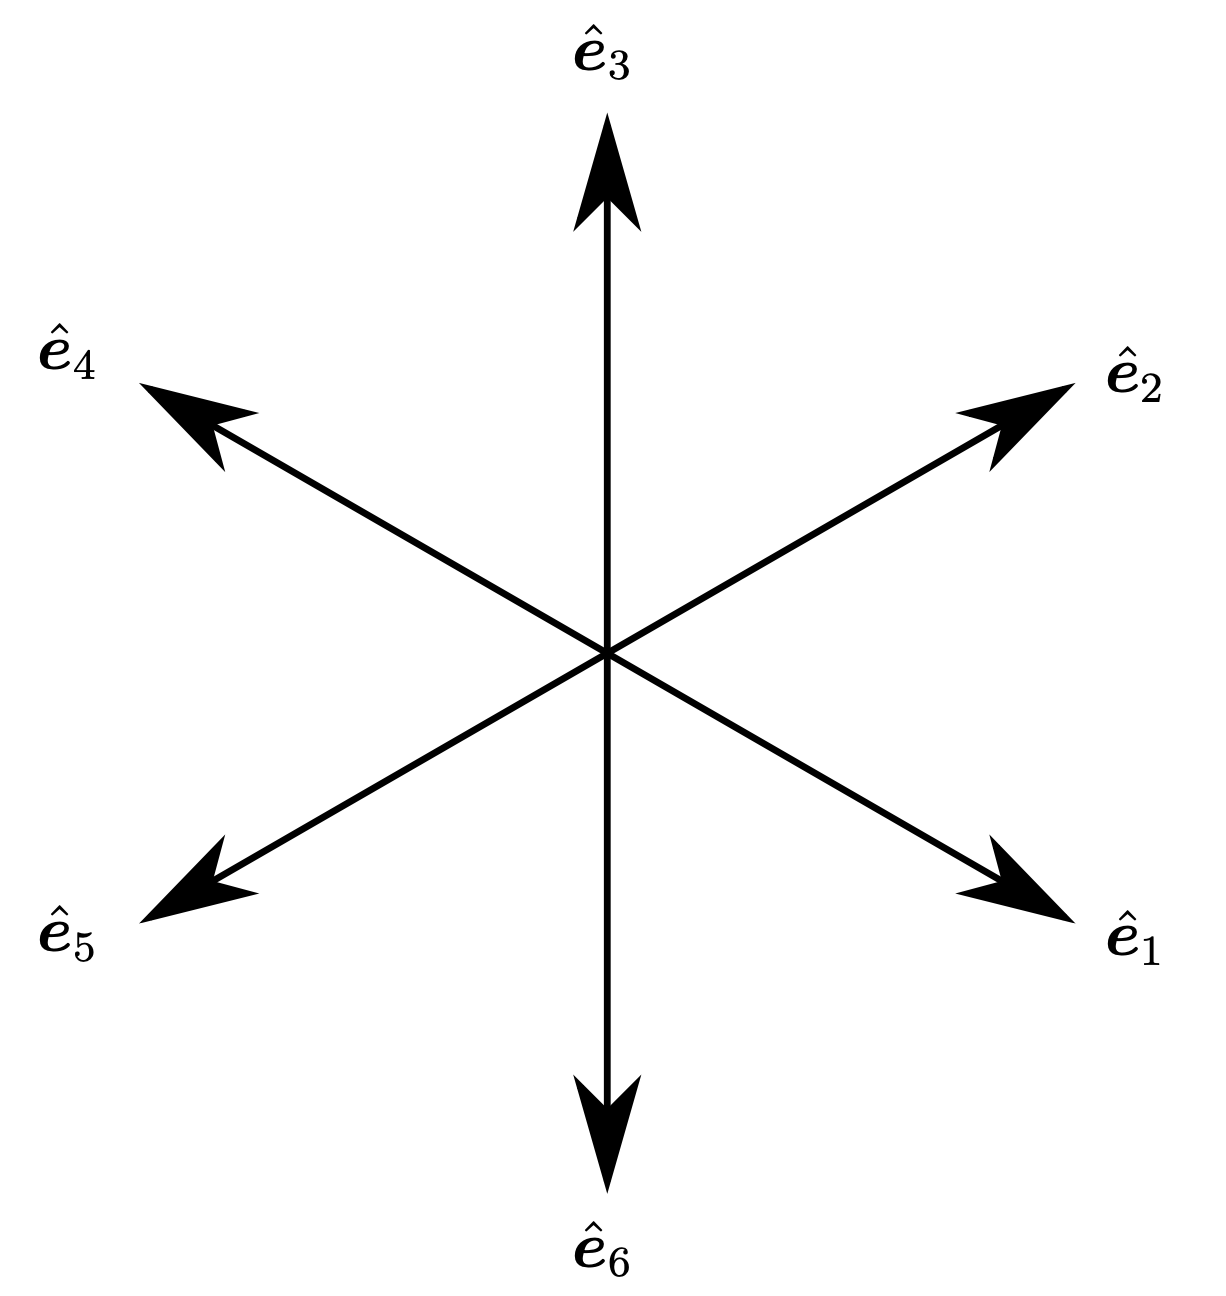
\includegraphics[width=0.5\columnwidth]{figures/LGA_lattice.png}
    \bicaption{二维速度空间中FPH模型的六边形格子,其包含有六个离散速度方向。}{Hexagonial lattice of the FHP model with six discrete velocity directions in two-dimensional velocity space.}
    \label{img:LGA_lattice}
\end{figure}

不论LGA或LBM,有一个通用的假设是,在一个时间步长$\Delta t$后,一个粒子会正好走过两个相邻格点间的距离$\Delta x$。对于一个六边形网格,有
\begin{equation}
    \mathbf{\xi}_i=\frac{\Delta x}{\Delta t}\hat{\mathbf{e}}_i,
\end{equation}
其中$\hat{\mathbf{e}}_i=\mathbf{e}_i/|\mathbf{e}_i|$是正则化后的粒子运动方向,$i$是速度方向的标号,$\mathbf{\xi}_i$是离散速度。那么接下来可以定义粒子的状态$n_{i}(\mathbf{x},t)$,这个状态值可以是0或1。不考虑碰撞的话,粒子的运动可以用方程描述:
\begin{equation}
    n_{i}(\mathbf{x}+\mathbf{\xi}_i \Delta t,t+\Delta t)=n_{i}(\mathbf{x},t).
    \label{eq:LGA}
\end{equation}
公式~\ref{eq:LGA}构成了LGA中标志性的迁移步骤。这一过程也被LBM所继承。这一点为LBM方法带来了很大的优势,首先就是线性的对流项大幅降低了计算难度。其次是这一种直接的空间离散形式并不需要生成一个特殊的计算网格,使前处理的复杂度也能大幅下降。然而这并不代表LBM对网格完全没有要求,这类基于格子的方法只能被应用于六边形或更常见的笛卡尔网格也是一种对网格的约束。

在LGA中,因为粒子只有两种状态,所以经常使用布尔 (Boolean) 变量表示。一般值为真 (true) 时表示在某个空间位置上有一个粒子正在以特定的速度移动,而值为假 (false) 时表示没有这样的粒子。这清楚地显示LGA方法是在粒子层面来表示流体的运动的~\cite{wolf2004lattice}。而很显然,想要完全真实地使用粒子来表示流体是不现实的,因为$1cm^3$的空气中就含有约$2.7\times 10^{19}$个粒子。这导致LGA只能采用比现实情况要低得多的粒子量进行仿真,使结果有很强的噪声。从而方法需要在空间和时间上进行平均才能取得相对正常的结果。为了解决这一问题,McNamara和Zanetti~(\citeyear{mcnamara1988use})提出使用一个表示粒子密度的分布函数来替代这种单个的粒子。这种抽象的表达也是玻尔兹曼输运方程 (Boltzmann Transport Equation, BTE) 的构成基础。所以被传输的值不再只是一个布尔值,而是一个实数。这个实数表达了在空间位置$\mathbf{x}$、时间$t$,找到一个速度为$\mathbf{\xi}$的粒子的概率的空间密度。那么在没有碰撞时的迁移步骤的方程变为:
\begin{equation}
    f_{i}(\mathbf{x}+\mathbf{\xi}_i \Delta t,t+\Delta t)=f_{i}(\mathbf{x},t),
    \label{eq:LBM_streaming}
\end{equation}
其中$f_{i}$是上述的概率分布函数,一般简称为分布函数。一般认为这标志着LBM的诞生。因为在微观过程上使用了统计的概念,所以LBM被称为介观 (mesoscopic) 方法。在公式~\ref{eq:LGA}与~\ref{eq:LBM_streaming}中,粒子间的交互被忽略了。考虑粒子间的交互,这个过程可以表示为
\begin{equation}
    f_{i}(\mathbf{x}+\mathbf{\xi}_i \Delta t,t+\Delta t)=f_{i}(\mathbf{x},t)+\Omega(f_{i}(\mathbf{x},t)),
    \label{eq:LBM_in_one}
\end{equation}
其中$\Omega$是碰撞运算符。然而在实际中,通常会将公式~\ref{eq:LBM_in_one}表示为两个分开的过程,即碰撞和迁移:
\begin{alignat}{2}
\textbf{碰撞:} & \quad\quad &f_i^*(\boldsymbol{x}, t) & =f_i(\boldsymbol{x}, t)+\Omega\left(f_i(\boldsymbol{x}, t)\right); \\
\textbf{迁移:} & & f_i\left(\boldsymbol{x}+\boldsymbol{\xi}_i \Delta t, t+\Delta t\right) & =f_i^*(\boldsymbol{x}, t),\label{eq:LBM_streaming_in_one}
\end{alignat}
其中,$f_i^*$表示碰撞后的分布函数。为了满足质量与动量守恒,LGA中的碰撞中设定了一些固定的规则。对于FHP模型来说,其只允许两个或三个粒子间的碰撞,并且粒子离开格点的方向不能和进入格点的方向一样。这使得两个粒子间的碰撞只有两种可能的结果,而三个粒子间的碰撞只有一种可能的结果,参见图~\ref{img:LGA_collision}。

\begin{figure}[htb]
    \centering
      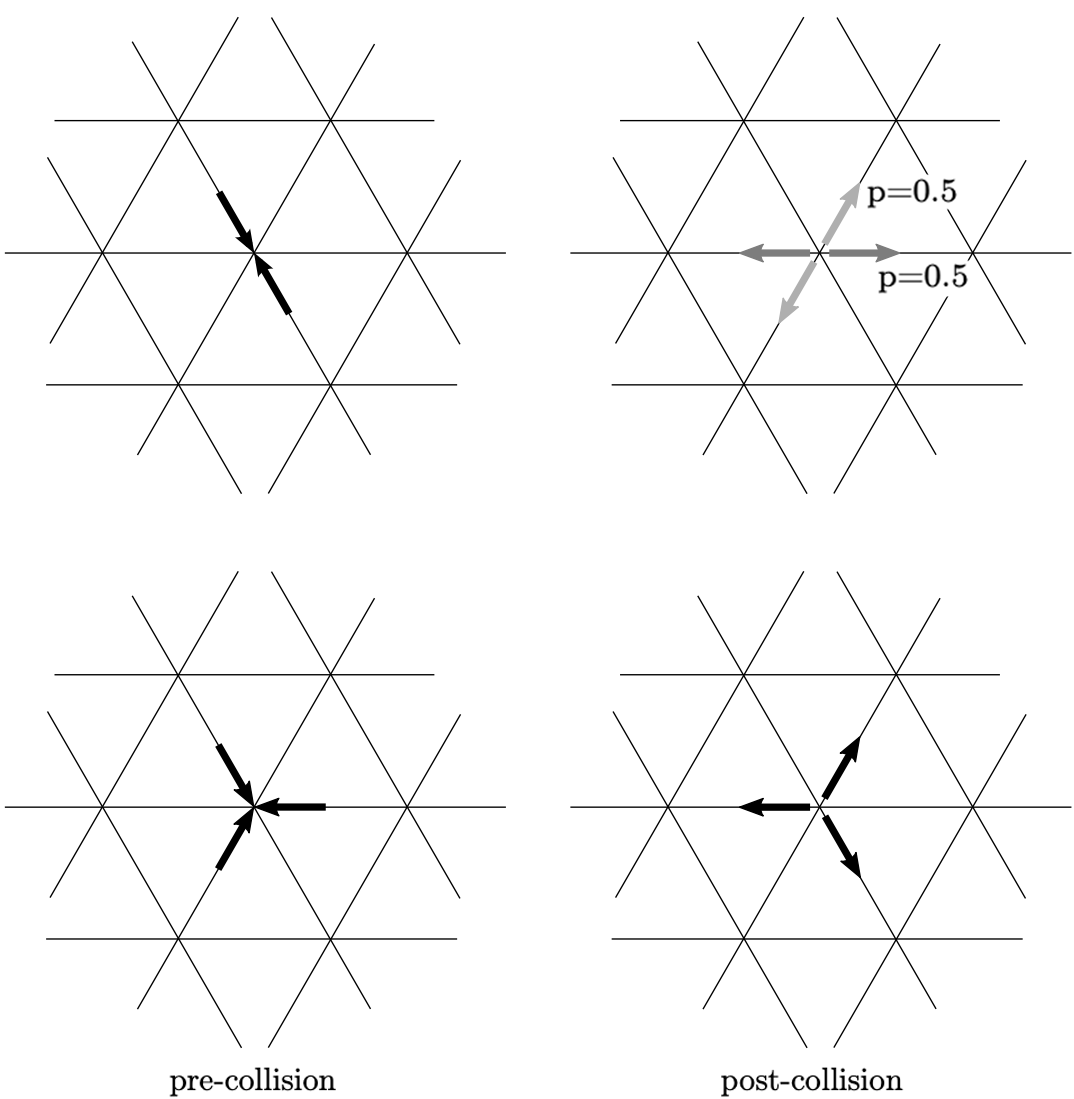
\includegraphics[width=0.9\columnwidth]{figures/LGA_collision.png}
    \bicaption{FHP模型中,两个粒子间的碰撞与三个粒子间的碰撞示意。$p$表示碰撞后的概率分布。}{Two- and three-particle collision in the FHP model. $p$ denotes the probablility of a particular post-collision state.}
    \label{img:LGA_collision}
\end{figure}

虽然,最初的LB模型也是基于这些碰撞规则,但是很快人们发现这样的碰撞规则不仅物理上不够精确,对于三维来说,所需的计算量也是不现实的。于是另一种增强的碰撞方案被提出~\cite{higuera1989lattice, higuera1989boltzmann},该方案将非线性的碰撞运算进行了线性化,使碰撞后的值与一个平衡态产生联系:
\begin{equation}
    \Omega(f_{i}(\mathbf{x}, t))=\mathbf{A}_{\alpha\beta}(f_{i}(\mathbf{x},t)+f_{i}^{eq}(\mathbf{x},t)),
\end{equation}
其中$\mathbf{A}$是一个散射矩阵 (scattering matrix),$f_{i}^{eq}$是离散的麦克斯韦-玻尔兹曼平衡态函数 (Maxwell-Boltzmann equilibrium function)。之后Qian等~(\citeyear{qian1992lattice}) 进一步对碰撞模型的简化,基本确定了现在最常见的LBM的碰撞形式,即粒子间的碰撞可以看作是分布函数向平衡态的一个松弛过程:
\begin{equation}
    \mathbf{A}=-\delta_{\alpha\beta}\tilde{\omega}.
\end{equation}
那么这个散射矩阵事实上可以被一个松弛系数$\tilde{\omega}$替代了,这个系数是松弛时间$\tilde{\tau}$的倒数:$\tilde{\omega}^{-1}=\tilde{\tau}=\frac{\tau}{\Delta t}$. 从而,公式~\ref{eq:LBM_in_one}变为
\begin{equation}
    f_{i}(\mathbf{x}+\mathbf{\xi}_i \Delta t,t+\Delta t)=f_{i}(\mathbf{x},t)-\tilde{\omega}(f_{i}(\mathbf{x},t)-f_{i}^{eq}(\mathbf{x},t)).
    \label{eq:LBM_in_one_BGK}
\end{equation}
现在所有的分布函数都以相同的速率向平衡态松弛,虽然这样非常地简洁高效,但是这种方法没有考虑对于分布函数中有物理意义和没有物理意义的部分是否需要分开处理。之后d'Humières~(\citeyear{d1992generalized}) 证明散射矩阵$\mathbf{A}$可以由一组特征基得到,这为多松弛时间模型的出现奠定了基础。

这种对碰撞本身的效果建模,而不是对微观过程建模的想法,最早可见于连续玻尔兹曼方程中的BGK碰撞模型~\cite{Bhatnagar-1954}。这个想法背后的动机是碰撞过程的大部分细节并不会对宏观量产生影响,所以可以将这些过程省略。除了质量与动量守恒之外,BGK模型还满足$\mathrm{H}$-定理,即分布函数会向平衡态趋近。基于BGK的LBM也是最简洁、最常见的LBM模型。


% Sec 2.2
\section{从介观量到宏观量}
对于大多数的流体应用,使用一组连续的状态量来描述,如速度、压力等一般已经足够。这些量其实是微观粒子状态的统计平均。在宏观上,流体可以被视为连续体并由N-S方程描述。然而LBM并非是一个宏观方法,而是介于微观与宏观之间的介观层面,如图~\ref{img:fluid_abstraction} 所示。

\begin{figure}[htb]
    \centering
      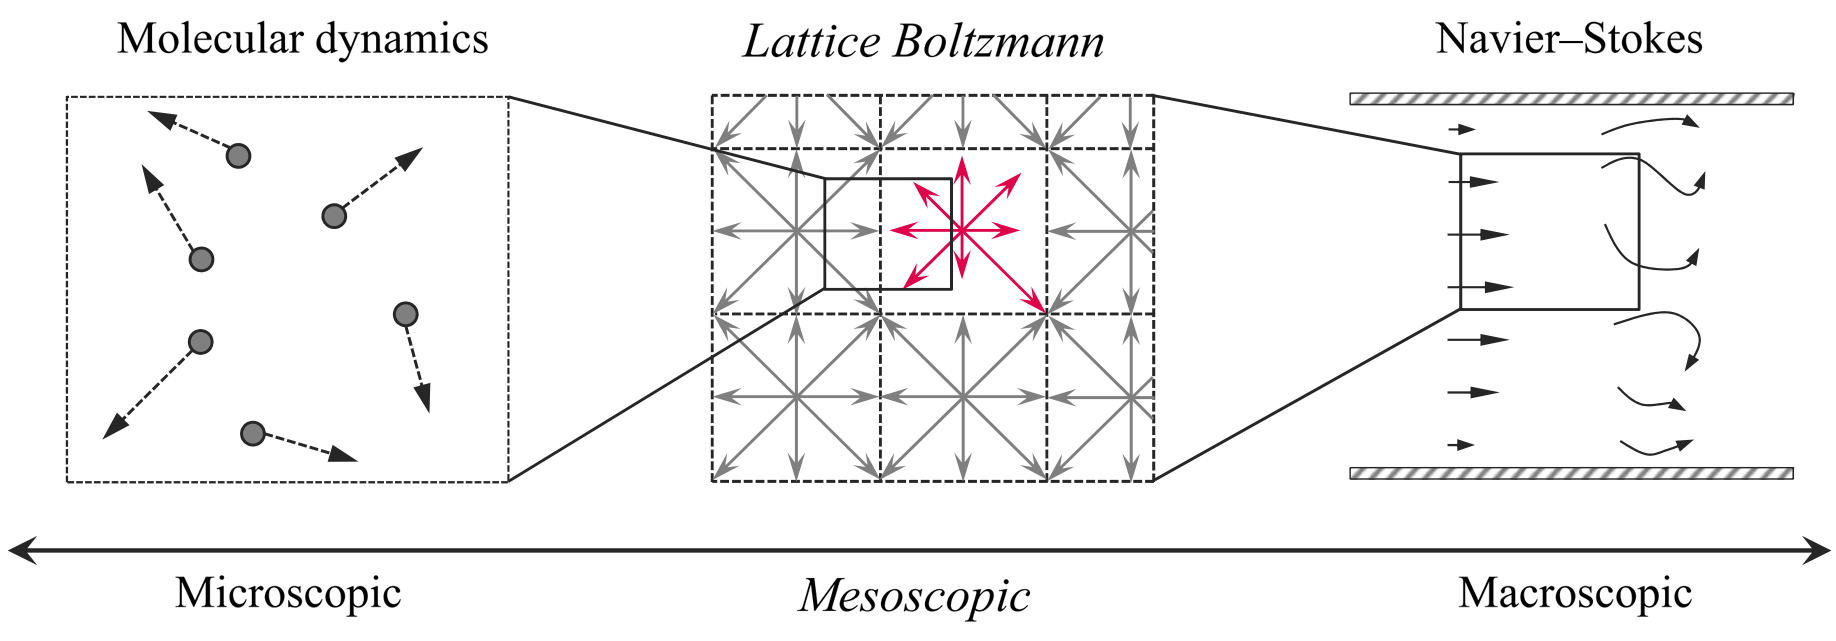
\includegraphics[width=0.9\columnwidth]{figures/fluid_abstraction.png}
    \bicaption{流体力学中的不同抽象层级。}{Different abstraction levels of the fluid dynamics.}
    \label{img:fluid_abstraction}
\end{figure}

可以认为LBM虽然采用了一种非常简化的方案,但它依然计算了部分的微观层面的交互。这也使得LBM的求解过程与N-S方程求解有本质的区别。然而我们最终目的依然是获取宏观的流体状态,以符合我们在宏观世界中对流体的感受。接下来我们将逐步介绍LBM中的概念,并建立其与宏观世界的联系。

可以认为,在一个给定的控制体积 (control volume) 中,分布函数表示了速度在$\boldsymbol{\xi}$与$\boldsymbol{\xi}+d\boldsymbol{\xi}$之间的粒子总数。所以宏观和介观值可以通过对速度空间$\boldsymbol{\Xi}$积分来建立联系,通过积分我们可以得到速度的n阶矩
\begin{equation}
    \boldsymbol{M}^{(n)}=\int_{\mathbb{R}^{\mathrm{D}}} \underbrace{\boldsymbol{\xi} \boldsymbol{\xi} \ldots \boldsymbol{\xi}}_{\mathrm{n} \text {次}} f(\boldsymbol{x}, \boldsymbol{\xi}, t) \mathrm{d} \boldsymbol{\xi},
\end{equation}
这里$D$代表积分的维度。在宏观层面,质量、动量和能量的守恒是由方程自身保证的,然而在介观层面,我们需要通过对碰撞运算符进行约束来保证,这个约束可以写作
\begin{equation}
    \int\left(\Omega(f) \cdot \psi\right) \mathrm{d} \boldsymbol{\xi}=0,
    \label{eq:collision_invariants}
\end{equation}
其中$\psi_k$是碰撞不变量 (collision invariants)。质量、动量和能量的守恒要求当$\psi=1, \boldsymbol{\xi}, |\boldsymbol{\xi}|^2$时,公式~\ref{eq:collision_invariants}是成立的。如果我们将碰撞不变量与分布函数的积进行积分,我们可以自然地得到连续速度空间中的宏观量
\begin{equation}
    \left\{\begin{array}{l}\rho(\boldsymbol{x}, t)=\int f(\boldsymbol{x}, \boldsymbol{\xi}, t) \mathrm{d} \boldsymbol{\xi} \\ \rho \boldsymbol{u}(\boldsymbol{x}, t)=\int \boldsymbol{\xi} f(\boldsymbol{x}, \boldsymbol{\xi}, t) \mathrm{d} \boldsymbol{\xi} \\ \rho E(\boldsymbol{x}, t)=\frac{1}{2} \int|\boldsymbol{\xi}|^2 f(\boldsymbol{x}, \boldsymbol{\xi}, t) \mathrm{d} \boldsymbol{\xi}\end{array}\right.,
\end{equation}
其中$E$为比能量 (specific energy)。对于单原子气体,碰撞可以假设为弹性的,所以比能量包含内能与动能
\begin{equation}
    \rho E=\rho\left(e+\frac{1}{2}|\boldsymbol{u}|^2\right).
\end{equation}
对于本动速度 (peculiar velocity) $\boldsymbol{v}=\boldsymbol{\xi}-\boldsymbol{u}$,即粒子在速度为$\boldsymbol{u}$的平均流中的相对速度,我们可以得到类似的公式:
\begin{equation}
    \rho e(\boldsymbol{x}, t)=\frac{1}{2} \int|\boldsymbol{v}|^2 f(\boldsymbol{x}, \boldsymbol{\xi}, t) \mathrm{d} \boldsymbol{\xi}.
\end{equation}
在连续概念的流体力学中,内能的守恒方程需要通过一个状态方程$p=p(\rho,e)$将压力和密度联系起来,即
\begin{equation}
    p=\frac{1}{\mathrm{D}} \int|\boldsymbol{v}|^2 f(\boldsymbol{x}, \boldsymbol{\xi}, t) \mathrm{d} \boldsymbol{\xi}=\frac{2}{\mathrm{D}} \rho e.
    \label{eq:eos}
\end{equation}
对于满足理想气体定律 (perfect gas law) 的等温流体,可以得到
\begin{equation}
    e=\frac{\mathrm{D}}{2} \frac{p}{\rho}=\frac{\mathrm{D}}{2} R T_0=\frac{\mathrm{D}}{2} \frac{k_B T_0}{m}=\frac{\mathrm{D}}{2} c_s^2,
\end{equation}
其中$T_0$和$c_s$分别表示常值的温度与声速,$k_B$是玻尔兹曼常数,$R$是气体常数。所以公式~\ref{eq:eos}可以被重写为
\begin{equation}
    p=\rho c_s^2,
\end{equation}
即绝热系数$\gamma=1$时的等熵状态方程~\cite{kundu2015fluid}。


% Sec 2.3
\section{速度空间的离散化}
如前文所述,由于在求解时保留了格子的概念,所以我们必须类似地对速度空间进行离散。分布函数事实上可以表达为Hermite多项式构成的无穷级数,变量为经过声速正则化后的速度空间$\tilde{\xi}=\xi/c_s$:
\begin{equation}
    f(\boldsymbol{x}, \boldsymbol{\xi}, t)=\frac{1}{c_s^{\mathrm{D}}} \omega(\tilde{\boldsymbol{\xi}}) \sum_{n=0}^{\infty} \frac{1}{n !} \boldsymbol{a}^{(n)}(\boldsymbol{x}, t) \mathscr{H}^{(n)}(\tilde{\boldsymbol{\xi}}),
    \label{eq:hermite_f}
\end{equation}
其中$\mathscr{H}^{(n)}$是$n$次多项式。Hermite多项式的一个特点是展开系数$\boldsymbol{a}^{(n)}$是$f$本身的速度矩~\cite{shan2006kinetic},权重函数$\omega$为
\begin{equation}
    \omega(\tilde{\boldsymbol{\xi}})=\frac{1}{(2 \pi)^{\mathrm{D} / 2}} \exp \left(-\tilde{\boldsymbol{\xi}}^2 / 2\right).
\end{equation}
当流体不受压力时,流体可以被一个平衡态函数描述。这只会出现在密度和速度在整个流体域中都是常值的情况下。此时的平衡态可由麦克斯韦分布函数描述
\begin{equation}
    f^{eq}=\frac{\rho}{\left(2 \pi c_s^2\right)^{\mathrm{D} / 2}} \exp \left(\frac{-(\boldsymbol{\xi}-\boldsymbol{u})^2}{2 c_s^2}\right),
    \label{eq:maxwell_eq}
\end{equation}
其中$\rho$和$\boldsymbol{u}$分别为宏观的密度和速度。我们可以将这个平衡态函数投影到基为Hermite多项式的空间,此时速度矩变为$\boldsymbol{a}^{eq,(n)}$:
\begin{equation}
    f^{eq}(\boldsymbol{x}, \boldsymbol{\xi}, t)=\frac{1}{c_s^{\mathrm{D}}} \omega(\tilde{\boldsymbol{\xi}}) \sum_{n=0}^{\infty} \frac{1}{n !} \boldsymbol{a}^{eq,(n)}(\boldsymbol{x}, t) \mathscr{H}^{(n)}(\tilde{\boldsymbol{\xi}}).
    \label{eq:maxwell_eq_hermite}
\end{equation}
对比公式~\ref{eq:maxwell_eq},我们可以注意到两式几乎有着相同的形式。事实上,$f^{eq}$还可表达为
\begin{equation}
    f^{eq}=\frac{\rho}{c_s^D}\omega(\tilde{\boldsymbol{v}}),
\end{equation}
其中$\tilde{\boldsymbol{v}}=(\boldsymbol{\xi})$可视为本动马赫数。所以麦克斯韦分布函数的Hermite展开系数为
\begin{equation}
    \boldsymbol{a}^{eq,(n)}=\rho \int w(\tilde{\boldsymbol{v}}) \mathscr{H}^{(n)}\left(\tilde{\boldsymbol{v}}+\frac{\boldsymbol{u}}{c_s}\right) \mathrm{d} \tilde{\boldsymbol{v}}.
    \label{eq:hermite_coefficients}
\end{equation}
对公式~\ref{eq:hermite_f}这样的无穷级数进行截断,即对应着对速度空间的离散化,并且保证了连续空间和离散空间下的矩在截断的阶数前是不变的。而离散的一个重要约束来自于高斯积分
\begin{equation}
    \int w(\boldsymbol{x}) f(\boldsymbol{x}) \mathrm{d} \boldsymbol{x} \approx \sum w_i f(\boldsymbol{x}_i), \quad i=0,1, \ldots, q-1
\end{equation}
其中,$f(\boldsymbol{x})$可表示任意函数而$\omega_i$是常值的权重。
%我们用$\tilde{\xi}_i$表达在$N$阶截断后的Hermite级数的横坐标 (abscissae),则高阶的截断一定会需要更多数量的离散速度,使格子的拓扑更难构造。
我们可以将高斯积分的公式抽象地记为
\begin{equation}
    E^q_{D,n},
\end{equation}
其中$D$表示空间的维度,$n$为积分精度的阶数,$q$表示积分所需要的离散点的数量。则我们可以推导出这三个值间的关系。对于一维空间,约束为$n>2N$并且$n=2q-1$~\cite{shan2006kinetic},所以可得$q=N+1$。对于高维空间并没有一般的高斯积分理论,但是我们可以假设有
\begin{equation}
    q=(N+1)^D.
\end{equation}
则二维的速度空间在$N=2$阶截断时需要9个离散速度,$N=3$时需要16个。当然实际的格子方向可能有所不同,因为考虑到某些矩的对称性,在维持$N$不变时所需的离散速度数量可能会减少。然而从几何上考虑,要设计能充满空间且各向同性的格子可能又会增加所需的格子方向数量。如果依然采用~\cite{qian1992lattice}中的D$d$Q$q$的命名的话,能维持二阶精度的格子分别为D1Q3、D2Q9、D3Q16。由公式~\ref{eq:hermite_coefficients}可得,在截断至二阶时,Hermite展开的系数为
\begin{equation}
    \left\{\begin{array}{l}\boldsymbol{a}^{eq, 0}=\rho \\ \boldsymbol{a}^{eq, 1}=\rho \frac{\boldsymbol{u}}{c_s} \\ \boldsymbol{a}^{eq, 2}=\rho \frac{u_i u_j}{c_s^2}\end{array}\right.
\end{equation}
将其代入到公式~\ref{eq:maxwell_eq_hermite}中,可以得到
\begin{equation}
    f_i^{eq}(\boldsymbol{x}, t)=w_i \rho\left(1+\frac{\boldsymbol{\xi}_i \cdot \boldsymbol{u}}{c_s^2}+\frac{\left(\boldsymbol{\xi}_i \cdot \boldsymbol{u}\right)^2}{2 c_s^4}-\frac{u^2}{2 c_s^2}\right),
    \label{eq:f_eq_o2}
\end{equation}
其中$f_i^{eq}(\boldsymbol{x}, t)=f^{eq}(\boldsymbol{x}, \xi_i, t)$, $\omega_i=\omega(\frac{\xi}{c_s})/c_s^D$。上述的推导尝试在尽量保持简洁的前提下,用比较系统且严格的形式推导出分布函数及速度空间的离散,所以无法过于详尽地展示出所有步骤。对于更彻底的推导,读者们可以参考~\cite{shan2006kinetic, malaspinas2010lattice}。


% Sec 2.4
\section{从LBM到N-S方程}
在介绍过速度矩作为介观和宏观世界之间的联系之后,我们现在将使用多尺度分析 (Multiple-scale Analysis) 来从LBE推导出N-S方程。许多流体的动态特征其实表现于其与平衡态的偏移。如果在介观上,分布函数都处于平衡态,那么可以想像,在宏观上流体也是平静的。所以多尺度分析的思想是将$f$在$f^{eq}$处展开。展开后的$f^{eq}$可以被记为$f^{(0)}$,其余部分为非平衡态项:
\begin{equation}
    f=\underbrace{f^{(0)}}_{f^{e q}}+\underbrace{\epsilon f^{(1)}+\epsilon^2 f^{(2)}}_{f^{n e q}} \cdots .
\end{equation}
多尺度分析的扩展依赖于一个很小的参数$\epsilon$,这个值是碰撞时间$\tau=\nu/c_s^2$与格子时间步长$\Delta t$的比值。对流的时间尺度 (advection timescale) 是直接与$\Delta t_1=\tau/\epsilon$联系的,而粘性扩散的时间尺度 ( viscous diffusion timescale) 是联系于
\begin{equation}
    \Delta t_2=\frac{\Delta x^2}{\nu} \sim \frac{c_s^2 \Delta t^2}{\nu}=\frac{\tau}{\epsilon^2}
    \label{eq:ms_f}
\end{equation}
的。有推导证明我们将$f$展开到一阶 ($\epsilon f^{(1)}$) 时,可以推导出欧拉方程~\cite{huang2008statistical}。为了推导N-S方程,我们需要展开到二阶 (即$\epsilon^2 f^{(2)}$),此时时间上的导数运算符为
\begin{equation}
    \frac{\partial}{\partial t}=\epsilon \frac{\partial}{\partial t_1}+\epsilon^2 \frac{\partial}{\partial t_2},
    \label{eq:ms_t}
\end{equation}
空间上的导数运算符为
\begin{equation}
    \frac{\partial}{\partial \boldsymbol{x}}=\epsilon \frac{\partial}{\partial \boldsymbol{x}_1}.
    \label{eq:ms_x}
\end{equation}
在将$f$分解为平衡态与非平衡态后,公式~\ref{eq:collision_invariants}所表达的约束可被表达为
\begin{equation}
    \sum_{i} f_{i}^{(n)}=\sum_{i} \boldsymbol{\xi}_{i} f_{i}^{(n)}=0, \quad  n=1,2, \ldots.
\end{equation}
那么为了将LBE恢复到N-S方程,首先我们要将公式~\ref{eq:LBM_in_one_BGK}的左手侧进行二阶的泰勒展开
\begin{align}
    \begin{split}
        & f_{i}\left(\boldsymbol{x}+\boldsymbol{\xi}_{i} \Delta t, t+\Delta t\right) \approx \\
        & \quad f_{i}(\boldsymbol{x}, t)+\left(\xi_{i \alpha} \Delta t \frac{\partial}{\partial x_{\alpha}}+\Delta t \frac{\partial}{\partial t}\right) f_{i}(\boldsymbol{x}, t)+ \\
        & \quad \frac{1}{2}\left(\xi_{i \alpha} \xi_{i \beta} \Delta t^{2} \frac{\partial^{2}}{\partial x_{\alpha} \partial x_{\beta}}+2 \xi_{i \alpha} \Delta t^{2} \frac{\partial}{\partial x_{\alpha}} \frac{\partial}{\partial t}+\Delta t^{2} \frac{\partial^{2}}{\partial t^{2}}\right) f_{i}(\boldsymbol{x}, t)+\mathcal{O}\left(\Delta t^{3}\right) .
    \end{split}
    \label{eq:ms_taylor}
\end{align}
我们将上式代入公式~\ref{eq:LBM_in_one_BGK},并用$\tau$替代$\tilde{\omega}$后,可以得到
\begin{equation}
\Delta t\left(\xi_{i \alpha} \frac{\partial}{\partial x_{\alpha}}+\frac{\partial}{\partial t}\right) f_{i}+\frac{\Delta t^{2}}{2}\left(\xi_{i \alpha} \xi_{i \beta} \frac{\partial^{2}}{\partial x_{\alpha} \partial x_{\beta}}+2 \xi_{i \alpha} \frac{\partial}{\partial x_{\alpha}} \frac{\partial}{\partial t}+\frac{\partial^{2}}{\partial t^{2}}\right) f_{i}=-\frac{\Delta t}{\tau}\left(f_{i}-f_{i}^{e q}\right) .
\end{equation}
接下来,我们将多尺度分析的公式~\ref{eq:ms_f}至~\ref{eq:ms_x}代入上式
\begin{align}
    \begin{split}
& {\left[\xi_{i \alpha}\left(\epsilon \frac{\partial}{\partial x_{1 \alpha}}\right)+\left(\epsilon \frac{\partial}{\partial t_{1}}+\epsilon^{2} \frac{\partial}{\partial t_{2}}\right)\right]\left(f_{i}^{(0)}+\epsilon f_{i}^{(1)}+\epsilon^{2} f_{i}^{(2)}\right)+} \\
& \frac{\Delta t}{2}\left[\xi_{i \alpha} \xi_{i \beta}\left(\epsilon^{2} \frac{\partial^{2}}{\partial x_{1 \alpha} \partial x_{1 \beta}}\right)+\left(2 \xi_{i \alpha} \epsilon^{2} \frac{\partial}{\partial x_{1 \alpha}} \frac{\partial}{\partial t_{1}}\right)+\left(\epsilon^{2} \frac{\partial^{2}}{\partial t_{1}^{2}}\right)\right]\left(f_{i}^{(0)}+\epsilon f_{i}^{(1)}+\epsilon^{2} f_{i}^{(2)}\right)= \\
& \quad-\frac{1}{\tau}\left(f_{i}^{(0)}+\epsilon f_{i}^{(1)}+\epsilon^{2} f_{i}^{(2)}-f_{i}^{e q}\right) .
    \end{split}
    \label{eq:ms_total}
\end{align}
接下来,我们把公式~\ref{eq:ms_total}按照$\epsilon$的阶数分离:

\noindent
$\mathcal{O}\left(\epsilon^{0}\right):$
\begin{equation}
f_{i}^{(0)}=f_{i}^{e q}
\end{equation}
$\mathcal{O}\left(\epsilon^{1}\right):$
\begin{equation}
\epsilon\left(\xi_{i \alpha} \frac{\partial}{\partial x_{1 \alpha}}+\frac{\partial}{\partial t_{1}}\right) f_{i}^{(0)}=-\frac{1}{\tau} \epsilon f_{i}^{(1)}
\label{eq:ms_o1}
\end{equation}
$\mathcal{O}\left(\epsilon^{2}\right):$
\begin{equation}
\epsilon^{2} \frac{\partial}{\partial t_{2}} f_{i}^{(0)}+\left(\xi_{i \alpha} \epsilon \frac{\partial}{\partial x_{1 \alpha}}+\epsilon \frac{\partial}{\partial t_{1}}\right) \epsilon f_{i}^{(1)}+\frac{\Delta t}{2}\left(\xi_{i \alpha} \epsilon \frac{\partial}{\partial x_{1 \alpha}}+\epsilon \frac{\partial}{\partial t_{1}}\right)^{2} f_{i}^{(0)}=-\frac{1}{\tau} \epsilon^{2} f_{i}^{(2)}
\label{eq:ms_o2}
\end{equation}
将公式~\ref{eq:ms_o1}代入公式~\ref{eq:ms_o2},可以得到
\begin{equation}
\epsilon^{2} \frac{\partial}{\partial t_{2}} f_{i}^{(0)}+\left(\xi_{i \alpha} \epsilon \frac{\partial}{\partial x_{1 \alpha}}+\epsilon \frac{\partial}{\partial t_{1}}\right)\left(1-\frac{\Delta t}{2 \tau}\right) \epsilon f_{i}^{(1)}=-\frac{1}{\tau} \epsilon^{2} f_{i}^{(2)}
\label{eq:ms_o1_into_o2}
\end{equation}
接下来我们想要获得关于宏观量的守恒公式,与求矩类似,我们对公式~\ref{eq:ms_o1}与公式~\ref{eq:ms_o1_into_o2}对碰撞不变量积分得到0阶与1阶的矩公式
\begin{equation}
\epsilon \frac{\partial \rho}{\partial t_{1}}+\epsilon \frac{\partial \rho u_{\alpha}}{\partial x_{1 \alpha}}=0,
\label{eq:ms_moment_o1_a}
\end{equation}
\begin{equation}
\epsilon \frac{\partial \rho u_{\alpha}}{\partial t_{1}}+\epsilon \frac{\partial P_{\alpha \beta}^{(0)}}{\partial x_{1 \beta}}=0,
\label{eq:ms_moment_o1_b}
\end{equation}
同样地,我们对公式~\ref{eq:ms_o2}积分得到矩公式
\begin{equation}
\epsilon^{2} \frac{\partial \rho}{\partial t_{2}} = 0,
\label{eq:ms_moment_o2_a}
\end{equation}
\begin{equation}
\epsilon^{2} \frac{\partial \rho u_{\alpha}}{\partial t_{2}} +\left(1-\frac{\Delta t}{2 \tau}\right) \epsilon^{2} \frac{P_{\alpha \beta}^{(1)}}{\partial x_{1 \beta}}=0 .
\label{eq:ms_moment_o2_b}
\end{equation}
然后我们将公式~\ref{eq:ms_moment_o1_a}与~\ref{eq:ms_moment_o1_b}相加,并将展开的求导运算符重新代回原式 (参见公式~\ref{eq:ms_t}与~\ref{eq:ms_x}) 可以得到
\begin{equation}
\frac{\partial \rho}{\partial t}+\frac{\partial \rho u_{\alpha}}{\partial x_{\alpha}}=0,
\end{equation}
即连续性方程。同样将公式~\ref{eq:ms_moment_o2_a}与~\ref{eq:ms_moment_o2_b}相加后得到
\begin{equation}
\frac{\partial \rho u_{\alpha}}{\partial t}+\frac{\partial}{\partial x_{\beta}}\left[P_{\alpha \beta}^{e q}+\left(1-\frac{\Delta t}{2 \tau}\right) P_{\alpha \beta}^{n e q}\right]=0,
\label{eq:ms_continuity_puzzle}
\end{equation}
其中$P_{\alpha \beta}^{e q}=P_{\alpha \beta}^{(0)}$,$P_{\alpha \beta}^{n e q}=P_{\alpha \beta}^{(1)}$。
由公式~\ref{eq:f_eq_o2}我们可以由下面的方式得到二阶矩
\begin{equation}
P_{\alpha \beta}^{(0)}=P_{\alpha \beta}^{e q}=\sum_{\alpha} f_{i}^{e q} \xi_{i, \alpha} \xi_{i, \beta}=\rho c_{s}^{2}\delta_{\alpha \beta}+\rho u_{\alpha} u_{\beta}.
\end{equation}
与三阶矩
\begin{equation}
Q_{\alpha \beta \gamma}^{(0)}=Q_{\alpha \beta \gamma}^{e q}=\sum_{\alpha} f_{i}^{e q} \xi_{i, \alpha} \xi_{i, \beta} \xi_{i, \gamma}=\rho c_{s}^{2}\left(u_{\alpha} \delta_{\beta \gamma}+u_{\beta} \delta_{\alpha \gamma}+u_{\gamma} \delta_{\alpha \beta}\right).
\end{equation}
那么在公式~\ref{eq:ms_continuity_puzzle}中,只剩下$P_{\alpha \beta}^{n e q}$是未知的。为了计算$P_{\alpha \beta}^{n e q}$,我们写出公式~\ref{eq:ms_o1}的2阶矩公式
\begin{equation}
\epsilon \frac{\partial P_{\alpha \beta}^{(0)}}{\partial t_{1}}+\epsilon \frac{\partial Q_{\alpha \beta \gamma}^{(0)}}{\partial x_{1 \gamma}}=-\frac{1}{\tau} \epsilon P_{\alpha \beta}^{(1)}.
\label{eq:ms_moment_o2}
\end{equation}
接下来,我们引入如下的积分公式 (乘积法则):
\begin{align}
\epsilon \frac{\partial \rho u_{\alpha} u_{\beta}}{\partial t_{1}} & =u_{\alpha} \epsilon \frac{\rho u_{\beta}}{\partial t_{1}}+u_{\beta} \epsilon \frac{\rho u_{\alpha}}{\partial t_{1}}-u_{\alpha} u_{\beta} \epsilon \frac{\partial \rho}{\partial t_{1}}, \\
\epsilon \frac{\partial \rho u_{\alpha} u_{\beta} u_{\gamma}}{\partial x_{1 \gamma}} & =u_{\alpha} \epsilon \frac{\rho u_{\beta} u_{\gamma}}{\partial x_{1 \gamma}}+u_{\beta} \epsilon \frac{\rho u_{\alpha} u_{\gamma}}{\partial x_{1 \gamma}}-u_{\alpha} u_{\beta} \epsilon \frac{\partial \rho u_{\gamma}}{\partial x_{1 \gamma}} .
\end{align}
使用上述的公式,公式~\ref{eq:ms_moment_o2}左手边的$\epsilon \frac{\partial P_{\alpha \beta}^{(0)}}{\partial t_{1}}$可以被表达为
\begin{align}
    \begin{split}
\epsilon \frac{\partial P_{\alpha \beta}^{(0)}}{\partial t_{1}}= & \epsilon \frac{\partial \rho u_{\alpha} u_{\beta}}{\partial t_{1}}+c_{s}^{2} \delta_{\alpha \beta} \epsilon \frac{\partial \rho}{\partial t_{1}} \\
= & u_{\alpha} \epsilon \frac{\partial \rho u_{\beta}}{\partial t_{1}}+u_{\beta} \epsilon \frac{\partial \rho u_{\alpha}}{\partial t_{1}}-u_{\alpha} u_{\beta} \epsilon \frac{\partial \rho}{\partial t_{1}}+c_{s}^{2} \delta_{\alpha \beta} \epsilon \frac{\partial \rho}{\partial t_{1}} \\
= & -u_{\alpha} \epsilon \frac{\partial P_{\beta \gamma}^{(0)}}{\partial x_{1 \gamma}}-u_{\beta} \epsilon \frac{\partial P_{\alpha \gamma}^{(0)}}{\partial x_{1 \gamma}}+u_{\alpha} u_{\beta} \epsilon \frac{\partial \rho u_{\gamma}}{\partial x_{1 \gamma}}-c_{s}^{2} \delta_{\alpha \beta} \epsilon \frac{\partial \rho u_{\gamma}}{\partial x_{1 \gamma}} \quad \text {(由公式~\ref{eq:ms_moment_o1_a}、\ref{eq:ms_moment_o1_b})} \\
= & -u_{\alpha} \epsilon \frac{\partial}{\partial x_{1 \gamma}}\left(\rho u_{\beta} u_{\gamma}+\rho c_{s}^{2} \delta_{\beta \gamma}\right)-u_{\beta} \epsilon \frac{\partial}{\partial x_{1 \gamma}}\left(\rho u_{\alpha} u_{\gamma}+\rho c_{s}^{2} \delta{\alpha \gamma}\right) \\
& +u_{\alpha} u_{\beta} \epsilon \frac{\partial \rho u_{\gamma}}{\partial x_{1 \gamma}}-c_{s}^{2} \delta_{\alpha \beta} \frac{\partial \rho u_{\gamma}}{\partial x_{1 \gamma}} \\
= & -\epsilon \frac{\partial \rho u_{\alpha} u_{\beta} u_{\gamma}}{\partial x_{1 \gamma}}-c_{s}^{2}\left(u_{\alpha} \epsilon \frac{\partial \rho}{\partial x_{1 \beta}}+u_{\beta} \epsilon \frac{\partial \rho}{\partial x_{1 \alpha}}\right)-c_{s}^{2} \delta_{\alpha \beta} \epsilon \frac{\partial \rho u_{\gamma}}{\partial x_{1 \gamma}} .
    \end{split}
\end{align}
同时,$\epsilon \frac{\partial Q_{\alpha \beta \gamma}^{(0)}}{\partial x_{1 \gamma}}$可表达为
\begin{align}
    \begin{split}
\epsilon \frac{\partial Q_{\alpha \beta \gamma}^{(0)}}{\partial x_{1 \gamma}} & =\epsilon \frac{\partial}{\partial x_{1 \gamma}} \rho c_{s}^{2}\left(u_{\alpha} \delta_{\beta \gamma}+u_{\beta} \delta{\alpha \gamma}+u_{\gamma} \delta_{\alpha \beta}\right) \\
& =c_{s}^{2}\left(\epsilon \frac{\partial \rho u_{\alpha}}{\partial x_{1 \beta}}+\epsilon \frac{\partial \rho u_{\beta}}{\partial x_{1 \alpha}}\right)+c_{s}^{2} \delta_{\alpha \beta} \epsilon \frac{\partial \rho u_{\gamma}}{\partial x_{1 \gamma}}.
    \end{split}
\end{align}
将上述两公式相加可得到$P_{\alpha \beta}^{(1)}$的表达式
\begin{equation}
\epsilon P_{\alpha \beta}^{(1)}=-\rho c_{s}^{2} \tau\left(\epsilon \frac{\partial u_{\alpha}}{\partial x_{1 \beta}}+\epsilon \frac{\partial u_{\beta}}{\partial x_{1 \alpha}}\right)+\tau \epsilon \frac{\partial \rho u_{\alpha} u_{\beta} u_{\gamma}}{\partial x_{1 \gamma}}.
\end{equation}
将 $P^{n e q}=\epsilon P^{(1)}$,$\partial / \partial \boldsymbol{x}=\epsilon \partial / \partial \boldsymbol{x}_{1}$代入,我们可以获得
\begin{equation}
P_{\alpha \beta}^{n e q}=\underbrace{-\rho c_{s}^{2} \tau\left(\frac{\partial u_{\alpha}}{\partial x_{\beta}}+\frac{\partial u_{\beta}}{\partial x_{\alpha}}\right)}_{\boldsymbol{\sigma}^{\prime}}+\underbrace{\tau \frac{\partial \rho u_{\alpha} u_{\beta} u_{\gamma}}{\partial x_{k}}}_{\text {误差项}} .
\label{eq:p_neq}
\end{equation}
从上式中我们可以发现,第一项对应于N-S方程中的粘性应力张量 (viscous stress tensor),第二项是误差项,因为平衡态函数$f_i^{eq}$只展开到了二阶,所以$\mathcal{O}\left(u^{3}\right)$项是不正确的。当我们仔细观察公式~\ref{eq:p_neq}时,我们发现当${u_x}^{2} \ll c_{s}^{2}$时,$\mathcal{O}\left(u^{3}\right)$项的模值相比前一项就可以被忽略了。所以在低马赫数时,我们可以直接忽略上式中的误差项。这也是为什么许多工作描述LBM只在弱可压情况下有效。
那么我们将忽略误差项的公式~\ref{eq:p_neq}代入公式~\ref{eq:ms_continuity_puzzle}后,可以得到动量守恒方程
\begin{equation}
    \frac{\partial \rho u_{\alpha}}{\partial t}+\frac{\partial \rho u_{\alpha} u_{\beta}}{\partial x_{\beta}}=-\frac{\partial p}{\partial x_{\alpha}}+\mu \frac{\partial}{\partial x_{\beta}}\left(\frac{\partial u_{\alpha}}{\partial x_{\beta}}+\frac{\partial u_{\beta}}{\partial x_{\alpha}}\right),
\end{equation}
其中$\mu=\left(1-\frac{\Delta t}{2 \tau}\right) \rho c_{s}^{2} \tau$是动力黏度 (dynamic viscosity),运动黏度 (kinematic viscosity) $\nu=\mu / \rho$与松弛时间$\tau$之间的关系为
\begin{equation}
    \nu=c_{s}^{2}\left(\tau-\frac{\Delta t}{2}\right) \quad \text {或} \quad \tau=\frac{\nu}{c_{s}^{2}}+\frac{\Delta t}{2} .
\end{equation}
因为我们在公式~\ref{eq:ms_taylor} 中对LBE进行了二阶的泰勒展开,所以我们认为在时间和空间上LBM可以以二阶的精度推导出N-S方程。


% Sec 2.5
\section{累积量碰撞模型}
在第~\ref{sec:2_LBM_origin} 节的末尾,我们介绍了LBM中的BGK碰撞模型 (即单松弛时间模型) 与多松弛时间模型出现的动机,并在第~\ref{sec:1_related_works_LBM} 节中介绍了基于不同量的MRT模型。在这些碰撞模型中,累积量碰撞模型相比其它模型 (原始矩、中心矩等) 有着遵守伽利略不变性、自由度耦合程度低、超黏度 (hyper-viscosity) 误差更小的优势,所以我们将基于累积量碰撞模型进行改进。在这里我们先简要的介绍累积量碰撞模型本身。

不同的碰撞模型的本质是在探索什么量可以最优地描述分布函数,我们称这些量为可观察量 (observable variables)。在累积量方法中,不同累积量之间是统计独立的 (statistically independent),也就是说,两个累积量的联合概率等于各自概率的积。为了推导出累积量,我们先将分布函数$f$转换到频率空间$F$中,这样便于我们进行泰勒展开。到频域的变换由拉普拉斯变换 (Laplace transform) 完成:
$$
F(\boldsymbol{\Xi})=\mathcal{L}\{f(\boldsymbol{\xi})\}.
$$
在三维中,我们令$\boldsymbol{\Xi}=\{\Xi, \Upsilon, \mathrm{Z}\}$,$\boldsymbol{\Xi}$代表了频率 (波数)。如果我们假设存在一个这样的可观察量$k_{\alpha\beta\gamma}$,使得它们的联合概率是它们各自概率的积
$$
F(\boldsymbol{\Xi})=\prod F_{\alpha \beta \gamma}\left(k_{\alpha \beta \gamma}\right).
$$
为了进行泰勒展开,我们对两边求对数,使等式右手边的积转为和
$$
\ln (F(\boldsymbol{\Xi}))=\sum \ln \left(F_{\alpha \beta \gamma}\left(k_{\alpha \beta \gamma}\right)\right),
$$
则函数$F$的变量$k_{\alpha \beta \gamma}$可被定义为累积量
$$
k_{\alpha \beta \gamma}=\left. \frac{\partial^{\alpha} \partial^{\beta} \partial^{\gamma}}{\partial \Xi^{\alpha} \partial \Upsilon^{\beta} \partial \mathrm{Z}^{\gamma}} \ln (F(\Xi, \Upsilon, \mathrm{Z}))\right|_{\Xi=\Upsilon=\mathrm{Z}=0}.
$$
我们称$k_{\alpha \beta \gamma}$是一个$n=\alpha+\beta+\gamma$阶的累积量。由上述推导,不同累积量是统计无关的,所以它们可以有各自不同的松弛系数
$$
k_{\alpha \beta \gamma}^{*}=\tilde{\omega}_{\alpha \beta \gamma} k_{\alpha \beta \gamma}^{e q}+\left(1-\tilde{\omega}_{\alpha \beta \gamma}\right) k_{\alpha \beta \gamma},
$$
其中$k_{\alpha \beta \gamma}^{*}$与$k_{\alpha \beta \gamma}^{eq}$分别表示碰撞后与平衡态的累积量。在这之后碰撞后的分布函数$f^*$可以由$k_{\alpha \beta \gamma}^{*}$得到。

接下来我们对于D3Q27格子的累积量LBM碰撞模型具体推导。在具体实现时,累积量碰撞过程可以分为五个阶段。第一个阶段是“前向中心矩变换”。虽然通过因为累积量的定义可以进行直接$f$到$k$的变换,但是这个计算过于复杂,而通过中心矩作为中间步骤计算累积量更为简单、有效,所以在实现中会先将$f$变换到中心矩$m$:
$$
m_{\alpha \beta \gamma} =\sum_{i,j,k} (i-u_x)^{\alpha} (j-u_y)^{\alpha} (k-u_z)^{\alpha} f_{ijk},
$$
其中$i, j, k \in \{-1, 0, 1\}$表示离散速度的方向,$\alpha, \beta, \gamma \in \{0, 1, 2\}$表示不同维度的阶数,$\boldsymbol{u}=\{u_x, u_y, u_z\}$表示宏观速度。因为中心矩变换是线性的,所以这个变换其实可以用一个矩阵$M$表示,则反向的变换可以用$M^{-1}$表示。但是我们注意到采用~\cite{Geier-2015}中的分方向的做法可以减少相当部分的计算量:
\begin{align*}
m_{i j \mid \gamma} & =\sum_{k} f_{ijk}(k-u_z)^{\gamma}, \\
m_{i \mid \beta \gamma} & =\sum_{j} m_{i j \mid \gamma}(j-u_y)^{\beta}, \\
m_{\alpha \beta \gamma} & =\sum_{i} m_{i \mid \beta \gamma}(i-u_x)^{\alpha}.
\end{align*}

得到中心矩后,第二个阶段为“前向累积量变换”。对于3阶及以下的累积量,其和中心矩相同:
\begin{align*}
& k_{110}=m_{110}, \\
& k_{200}=m_{200}, \\
& k_{120}=m_{120}, \\
& k_{111}=m_{111} .
\end{align*}
对于$k_{101}$与$k_{020}$等同阶的累积量,可以将上述的对应公式的变量下标交换位置得到。4阶及以上的累积量可通过如下公式得到:
\begin{align*}
k_{211} & =m_{211}-\left(m_{200} m_{011}+2 m_{110} m_{101}\right) / \rho \\
k_{220} & =m_{220}-\left(m_{200} m_{020}+2 m_{110}^{2}\right) / \rho \\
k_{122} & =m_{122}-\left(m_{002} m_{120}+m_{020} m_{102}+4 m_{011} m_{111}+2\left(m_{101} m_{021}+m_{110} m_{012}\right)\right) / \rho \\
k_{222} & =m_{222}-\left(4 m_{111}^{2}+m_{200} m_{022}+m_{020} m_{202}+m_{002} m_{220}\right. \\
&\quad +4\left(m_{011} m_{211}+m_{101} m_{121}+m_{110} m_{112}\right) \\
&\quad \left.+2\left(m_{120} m_{102}+m_{210} m_{012}+m_{201} m_{021}\right)\right) / \rho \\
&\quad +\left(16 m_{110} m_{101} m_{011}+4\left(m_{101}^{2} m_{020}+m_{011}^{2} m_{200}+m_{110}^{2} m_{002}\right)\right. \\
&\quad \left.+2 m_{200} m_{020} m_{002}\right) / \rho^{2} ,
\end{align*}
对于同阶的累积量,同样可以将上述的对应公式的变量下标交换位置得到。

第三个阶段是“碰撞”。首先二阶累积量的碰撞公式如下:
\begin{align*}
& k_{110}^{*}=\left(1-\omega_{1}\right) k_{110}, \\
& k_{101}^{*}=\left(1-\omega_{1}\right) k_{101}, \\
& k_{011}^{*}=\left(1-\omega_{1}\right) k_{011} ,
\end{align*}
其中含星号的变量代表碰撞后的变量。这些累积量的平衡态为0,所以被省去。而由于格子离散化时的各向异性,有些累积量并不为0:
\begin{align*}
k_{200}^{*}-k_{020}^{*} & =\left(1-\omega_{1}\right)\left(k_{200}-k_{020}\right)-3 \rho\left(1-\frac{\omega_{1}}{2}\right)\left({u_x}^{2} \frac{\partial u_x}{\partial x}-{u_y}^{2} \frac{\partial u_y}{\partial y}\right), \\
k_{200}^{*}-k_{002}^{*} & =\left(1-\omega_{1}\right)\left(k_{200}-k_{002}\right)-3 \rho\left(1-\frac{\omega_{1}}{2}\right)\left({u_x}^{2} \frac{\partial u_x}{\partial x}-{u_z}^{2} \frac{\partial u_z}{\partial z}\right), \\
k_{200}^{*}+k_{020}^{*}+k_{002}^{*} & =\kappa_{000} \omega_{2}+\left(1-\omega_{2}\right)\left(k_{200}+k_{020}+k_{002}\right) \\
&\quad -3 \rho\left(1-\frac{\omega_{2}}{2}\right)\left({u_x}^{2} \frac{\partial u_x}{\partial x}+{u_y}^{2} \frac{\partial u_y}{\partial y}+{u_z}^{2} \frac{\partial u_z}{\partial z}\right) ,
\end{align*}
其中速度的梯度部分可由二阶的累积量计算得到:
\begin{align*}
\frac{\partial u_x}{\partial x} & =-\frac{\omega_{1}}{2 \rho}\left(2 k_{200}-k_{020}-k_{002}\right)-\frac{\omega_{2}}{2 \rho}\left(k_{200}+k_{020}+k_{002}-\kappa_{000}\right), \\
\frac{\partial u_y}{\partial y} & =\frac{\partial u_x}{\partial x}+\frac{3 \omega_{1}}{2 \rho}\left(k_{200}-k_{020}\right), \\
\frac{\partial u_z}{\partial z} & =\frac{\partial u_x}{\partial x}+\frac{3 \omega_{1}}{2 \rho}\left(k_{200}-k_{002}\right), \\
\frac{\partial u_y}{\partial x}+\frac{\partial u_x}{\partial y} & =-\frac{3 \omega_{1}}{\rho} k_{110}, \\
\frac{\partial u_z}{\partial x}+\frac{\partial u_x}{\partial z} & =-\frac{3 \omega_{1}}{\rho} k_{101}, \\
\frac{\partial u_z}{\partial y}+\frac{\partial u_y}{\partial z} & =-\frac{3 \omega_{1}}{\rho} k_{011}.
\end{align*}
剩余部分的碰撞公式为:
\begin{align*}
k_{120}^{*}+k_{102}^{*} & =\left(1-\omega_{3}\right)\left(k_{120}+k_{102}\right), \\
k_{210}^{*}+k_{012}^{*} & =\left(1-\omega_{3}\right)\left(k_{210}+k_{012}\right), \\
k_{201}^{*}+k_{021}^{*} & =\left(1-\omega_{3}\right)\left(k_{201}+k_{021}\right), \\
k_{120}^{*}-k_{102}^{*} & =\left(1-\omega_{4}\right)\left(k_{120}-k_{102}\right), \\
k_{210}^{*}-k_{012}^{*} & =\left(1-\omega_{4}\right)\left(k_{210}-k_{012}\right), \\
k_{201}^{*}-k_{021}^{*} & =\left(1-\omega_{4}\right)\left(k_{201}-k_{021}\right), \\
k_{111}^{*} & =\left(1-\omega_{5}\right) k_{111}, \\
k_{220}^{*}-2 k_{202}^{*}+k_{022}^{*} & =\frac{2}{3}\left(\frac{1}{\omega_{1}}-\frac{1}{2}\right) \omega_{6} A \rho\left(\frac{\partial u_x}{\partial x}-2 \frac{\partial u_y}{\partial y}+\frac{\partial u_z}{\partial z}\right) \\
&\quad +\left(1-\omega_{6}\right)\left(k_{220}-2 k_{202}+k_{022}\right), \\
k_{220}^{*}+k_{202}^{*}-2 k_{022}^{*} & =\frac{2}{3}\left(\frac{1}{\omega_{1}}-\frac{1}{2}\right) \omega_{6} A \rho\left(\frac{\partial u_x}{\partial x}+\frac{\partial u_y}{\partial y}-2 \frac{\partial u_z}{\partial z}\right) \\
&\quad +\left(1-\omega_{6}\right)\left(k_{220}+k_{202}-2 k_{022}\right), \\
k_{220}^{*}+k_{202}^{*}+k_{022}^{*} & =-\frac{4}{3}\left(\frac{1}{\omega_{1}}-\frac{1}{2}\right) \omega_{7} A \rho\left(\frac{\partial u_x}{\partial x}+\frac{\partial u_y}{\partial y}+\frac{\partial u_z}{\partial z}\right) \\
&\quad +\left(1-\omega_{7}\right)\left(k_{220}+k_{202}+k_{022}\right), \\
k_{211}^{*} & =-\frac{1}{3}\left(\frac{1}{\omega_{1}}-\frac{1}{2}\right) \omega_{8} B \rho\left(\frac{\partial u_z}{\partial y}+\frac{\partial u_y}{\partial z}\right)+\left(1-\omega_{8}\right) k_{211}, \\
k_{121}^{*} & =-\frac{1}{3}\left(\frac{1}{\omega_{1}}-\frac{1}{2}\right) \omega_{8} B \rho\left(\frac{\partial u_z}{\partial x}+\frac{\partial u_x}{\partial z}\right)+\left(1-\omega_{8}\right) k_{121}, \\
k_{112}^{*} & =-\frac{1}{3}\left(\frac{1}{\omega_{1}}-\frac{1}{2}\right) \omega_{8} B \rho\left(\frac{\partial u_y}{\partial x}+\frac{\partial u_x}{\partial y}\right)+\left(1-\omega_{8}\right) k_{112}, \\
k_{221}^{*} & =\left(1-\omega_{9}\right) k_{221}, \\
k_{212}^{*} & =\left(1-\omega_{9}\right) k_{212}, \\
k_{122}^{*} & =\left(1-\omega_{9}\right) k_{122}, \\
k_{222}^{*} & =\left(1-\omega_{10}\right) k_{222} .
\end{align*}
可以看到,4阶的累积量中有$A$和$B$两个参数变量,这两个参数变量源于~\cite{Geier-2017}中的对4阶累积量参数化,这个参数化的目的是消除线性的领头误差 (linearized leading error),从而提高求解精度。在优化后,三阶累积量的松弛系数与$A$、$B$可以被确定为
\begin{align*}
\omega_{3} =& \frac{8\left(\omega_{1}-2\right)\left(\omega_{2}\left(3 \omega_{1}-1\right)-5 \omega_{1}\right)}{8\left(5-2 \omega_{1}\right) \omega_{1}+\omega_{2}\left(8+\omega_{1}\left(9 \omega_{1}-26\right)\right)} \\
\omega_{4} =& \frac{8\left(\omega_{1}-2\right)\left(\omega_{1}+\omega_{2}\left(3 \omega_{1}-7\right)\right)}{\omega_{2}\left(56-42 \omega_{1}+9 \omega_{1}^{2}\right)-8 \omega_{1}} \\
\omega_{5} =& \frac{24\left(\omega_{1}-2\right)\left(4 \omega_{1}^{2}+\omega_{1} \omega_{2}\left(18-13 \omega_{1}\right)+\omega_{2}^{2}\left(2+\omega_{1}\left(6 \omega_{1}-11\right)\right)\right)}{16 \omega_{1}^{2}\left(\omega_{1}-6\right)-2 \omega_{1} \omega_{2}\left(216+5 \omega_{1}\left(9 \omega_{1}-46\right)\right)+\omega_{2}^{2}\left(\omega_{1}\left(3 \omega_{1}-10\right)\left(15 \omega_{1}-28\right)-48\right)}, \\
A =& \frac{4 \omega_{1}^{2}+2 \omega_{1} \omega_{2}\left(\omega_{1}-6\right)+\omega_{2}^{2}\left(\omega_{1}\left(10-3 \omega_{1}\right)-4\right)}{\left(\omega_{1}-\omega_{2}\right)\left(\omega_{2}\left(2+3 \omega_{1}\right)-8 \omega_{1}\right)}, \\
B = & \frac{4 \omega_{1} \omega_{2}\left(9 \omega_{1}-16\right)-4 \omega_{1}^{2}-2 \omega_{2}^{2}\left(2+9 \omega_{1}\left(\omega_{1}-2\right)\right)}{3\left(\omega_{1}-\omega_{2}\right)\left(\omega_{2}\left(2+3 \omega_{1}\right)-8 \omega_{1}\right)} .
\end{align*}
由于$\omega_{2}$在累积量碰撞模型中是用来控制体积黏度 (bulk viscosity) 的,为了简化,我们可以将$\omega_{2}$设置为1,则上述公式简化为
\begin{align*}
    \omega_{3} =& \frac{8\left(\omega_{1}-2\right)\left(1+2 \omega_{1}\right)}{-8-14\omega_{1}+7\omega_{1}^2} \\
    \omega_{4} =& \frac{8\left(\omega_{1}-2\right)\left(4 \omega_{1}-7\right)}{56-50\omega_{1}+9\omega_{1}^2} \\
    \omega_{5} =& \frac{24\left(\omega_{1}-2\right)\left(-2-7\omega_{1}+3\omega_{1}^2\right)}{48+152\omega_{1}-130\omega_{1}^2+29\omega_{1}^3}, \\
    A =& \frac{4+2\omega_{1}-3\omega_{1}^2}{2-7\omega_{1}+5\omega_{1}^2}, \\
    B =& \frac{4+28\omega_{1}-14\omega_{1}^2}{6-21\omega_{1}+15\omega_{1}^2} .
\end{align*}

第四个阶段是“后向累积量变换”:
\begin{align*}
m_{211}^{*}= & k_{211}^{*}+\left(m_{200}^{*} m_{011}^{*}+2 m_{110}^{*} m_{101}^{*}\right) / \rho \\
m_{220}^{*}= & k_{220}^{*}+\left(m_{200}^{*} m_{020}^{*}+2 m_{110}^{* 2}\right) / \rho \\
m_{122}^{*}= & k_{122}^{*}+\left(m_{002}^{*} m_{120}^{*}+m_{020}^{*} m_{102}^{*}+4 m_{011}^{*} m_{111}^{*}+2\left(m_{101}^{*} m_{021}^{*}+m_{110}^{*} m_{012}^{*}\right)\right) / \rho \\
m_{222}^{*}= & k_{222}^{*}+\left(4 m_{111}^{* 2}+m_{200}^{*} m_{022}^{*}+m_{020}^{*} m_{202}^{*}+m_{002}^{*} m_{220}^{*}\right. \\
& +4\left(m_{011}^{*} m_{211}^{*}+m_{101}^{*} m_{121}^{*}+m_{110}^{*} m_{112}^{*}\right) \\
& \left.+2\left(m_{120}^{*} m_{102}^{*}+m_{210}^{*} m_{012}^{*}+m_{201}^{*} m_{021}^{*}\right)\right) / \rho \\
& -\left(16 m_{110}^{*} m_{101}^{*} m_{011}^{*}+4\left(m_{101}^{* 2} m_{020}^{*}+m_{011}^{* 2} m_{200}^{*}+m_{110}^{* 2} m_{002}^{*}\right)\right. \\
& \left.+2 m_{200}^{*} m_{020}^{*} m_{002}^{*}\right) / \rho^{2} .
\end{align*}
这是“前向累积量变换”的逆过程,对于同阶的累积量,可以将上述的对应公式的变量下标交换位置得到。

第五个阶段是“后向中心矩变换”。这里我们同样采用~\cite{Geier-2015}中的做法来减少计算量:
\begin{align*}
    & m_{0 \mid \beta \gamma}^{*}=m_{0 \beta \gamma}^{*}\left(1-u_x^{2}\right)-2u_x m_{1 \beta \gamma}^{*}-m_{2 \beta \gamma}^{*}, \\
    & m_{\overline{1} \mid \beta \gamma}^{*}=\left(m_{0 \beta \gamma}^{*}\left(u_x^{2}-u_x\right)+m_{1 \beta \gamma}^{*}(2 u_x-1)+m_{2 \beta \gamma}^{*}\right) / 2, \\
    & m_{1 \mid \beta \gamma}^{*}=\left(m_{0 \beta \gamma}^{*}\left(u_x^{2}+u_x\right)+m_{1 \beta \gamma}^{*}(2 u_x+1)+m_{2 \beta \gamma}^{*}\right) / 2, \\
    & m_{i 0 \mid \gamma}^{*}=m_{i \mid 0 \gamma}^{*}\left(1-u_y^{2}\right)-2u_y m_{i \mid 1 \gamma}^{*}-m_{i \mid 2 \gamma}^{*}, \\
    & m_{i \overline{1} \mid \gamma}^{*}=\left(m_{i \mid 0 \gamma}^{*}\left(u_y^{2}-u_y\right)+m_{i \mid 1 \gamma}^{*}(2 u_y-1)+m_{i \mid 2 \gamma}^{*}\right) / 2, \\
    & m_{i 1 \mid \gamma}^{*}=\left(m_{i \mid 0 \gamma}^{*}\left(u_y^{2}+u_y\right)+m_{i \mid 1 \gamma}^{*}(2 u_y+1)+m_{i \mid 2 \gamma}^{*}\right) / 2, \\
    & f_{i j 0}^{*}=m_{i j \mid 0}^{*}\left(1-u_z^{2}\right)-2u_z m_{i j \mid 1}^{*}-m_{i j \mid 2}^{*}, \\
    & f_{i j \overline{1}}^{*}=\left(m_{i j \mid 0}^{*}\left(u_z^{2}-u_z\right)+m_{i j \mid 1}^{*}(2 u_z-1)+m_{i j \mid 2}^{*}\right) / 2, \\
    & f_{i j 1}^{*}=\left(m_{i j \mid 0}^{*}\left(u_z^{2}+u_z\right)+m_{i j \mid 1}^{*}(2 u_z+1)+m_{i j \mid 2}^{*}\right) / 2 .
\end{align*}
    

% Sec 2.6
\section{边界处理}
\label{sec:boundary_treatment}
显然,在公式~\ref{eq:LBM_streaming_in_one} 所描述的迁移过程中,分布函数可以顺利移动的一个原因是,流体中并没有任何固体的阻碍。
那么当流体附近存在固体时,边界处理是必须的。如图~\ref{img:bounce_back_scheme} 中,对于流体点$\bm{x}_b$,存在速度方向$\bm{l}_j$,使得邻点$\bm{x}_b-\bm{l}_j$位于固体内部。这会导致$\bm{l}_j'$方向的分布函数无法通过正常迁移得到,从而必须需要边界处理方法进行构造。
LBM的边界处理有一定的复杂性,其中一个主要来源是,因为LBM普遍使用笛卡尔网格,所以边界通常是落在格点之外的位置。针对这个问题在实际应用中有两类边界处理方法,分别是基于格点的 (node-based) 和方向性的 (directional)。基于格点的方法会根据边界的位置和其它信息来一次性修改所有方向的分布函数,而方向性方法只会修改未知方向的分布函数。

由于在LBM中有着非常多的边界处理形式,我们在这里回顾一些跟当前工作最相关的边界处理方法。

\subsection{浸入边界法}
浸入边界法 (immersed boundary method,IBM) 是一个在LBM被经常采用的边界处理方法,其一般通过施加惩罚力实现边界条件~\cite{patel2018diffuse,mittal-2008,Li-2020}。在浸入边界法的诸多变种中,锐利界面浸入边界法 (sharp-interface immersed boundary, SI-IBM)~\cite{mittal-2008} 是最为精准的。该方法的图示可见图~\ref{img:bounce_back_scheme}。
对于边界点,SI-IBM首先重建相邻固体点的分布函数 (在图~\ref{img:bounce_back_scheme} 中标为方框)。之后将该格点投影到固体边界上 (在图~\ref{img:bounce_back_scheme} 中标为$\bm{p}^\perp$),然后沿着法向$\bm{p}^\perp\!-\!\bm{p}$方向求得一个镜像点$\bm{p}'$。$\bm{p}'$的宏观速度可在固体边界的一侧通过周围点插值得到。因为固体点的速度$\bm{u}_b(\bm{p}^\perp)$是已知的,我们可以容易地计算出$\bm{p}$点的速度$\bm{u}^*(\bm{p}) = 2\bm{u}_b(\bm{p}^\perp) - \bm{u}(\bm{p}')$。显然这个速度会与$\bm{p}$点现有的宏观速度$\bm{u}(\bm{p})$有一个速度差$\Delta\bm{u}(\bm{p}) = \bm{u}^*(\bm{p}) - \bm{u}(\bm{p})$。这个速度差可以构成一个惩罚力$\bm{F}(\bm{p}) = \rho\Delta\bm{u}(\bm{p})$来修正$\bm{p}$点的流体速度。

SI-IBM的一个优势是通过插值,固体边界的大速度梯度会被压制,从而提升稳定性。但是由于它需求有固体内部点参与计算,对于亚网格尺度的物体,SI-IBM并不适合。这一点在第\ref{sec:siga21}章中有更详细的说明。同时,在物体运动时,SI-IBM需要格点重填 (node refilling),这会引入速度外插之外的新的误差。

\subsection{简单反弹边界}
简单反弹边界在LBM中同样有着重要的地位,不仅因为它是最早被应用在LBM中的边界处理方法之一,也因为其非常简洁的构造被广泛使用。对于未知的分布函数,简单反弹边界通过一个事实上的“反弹”来构造未知的分布函数:
\begin{equation}\label{eq:bounce-back}
f_{j}(\bm{x},t+1) = f_{j'}(\bm{x},t) - 6 w_{j}\rho\bm{u}_s \cdot \bm{c}_{j}\;,
\end{equation}
其中$j'$是与$j$相反的速度方向序号,即$\bm{c}_{j'}\!=\!-\bm{c}_j$;$w_j$是速度方向权重,$\bm{u}_s$是线段$\bm{x}_b$至$\bm{x}_b-\bm{c}_{j'}$与边界交点的速度。
然而,简单反弹边界的简洁也带来了一些局限性。因为分布函数永远假设在速度方向的中间被反弹,这会产生较大的速度梯度与色散误差,并给高雷诺数湍流仿真带来很强的不稳定性。这一点同样在第\ref{sec:siga21}章中有更详细的说明。

\begin{figure}[htb]
    \centering
      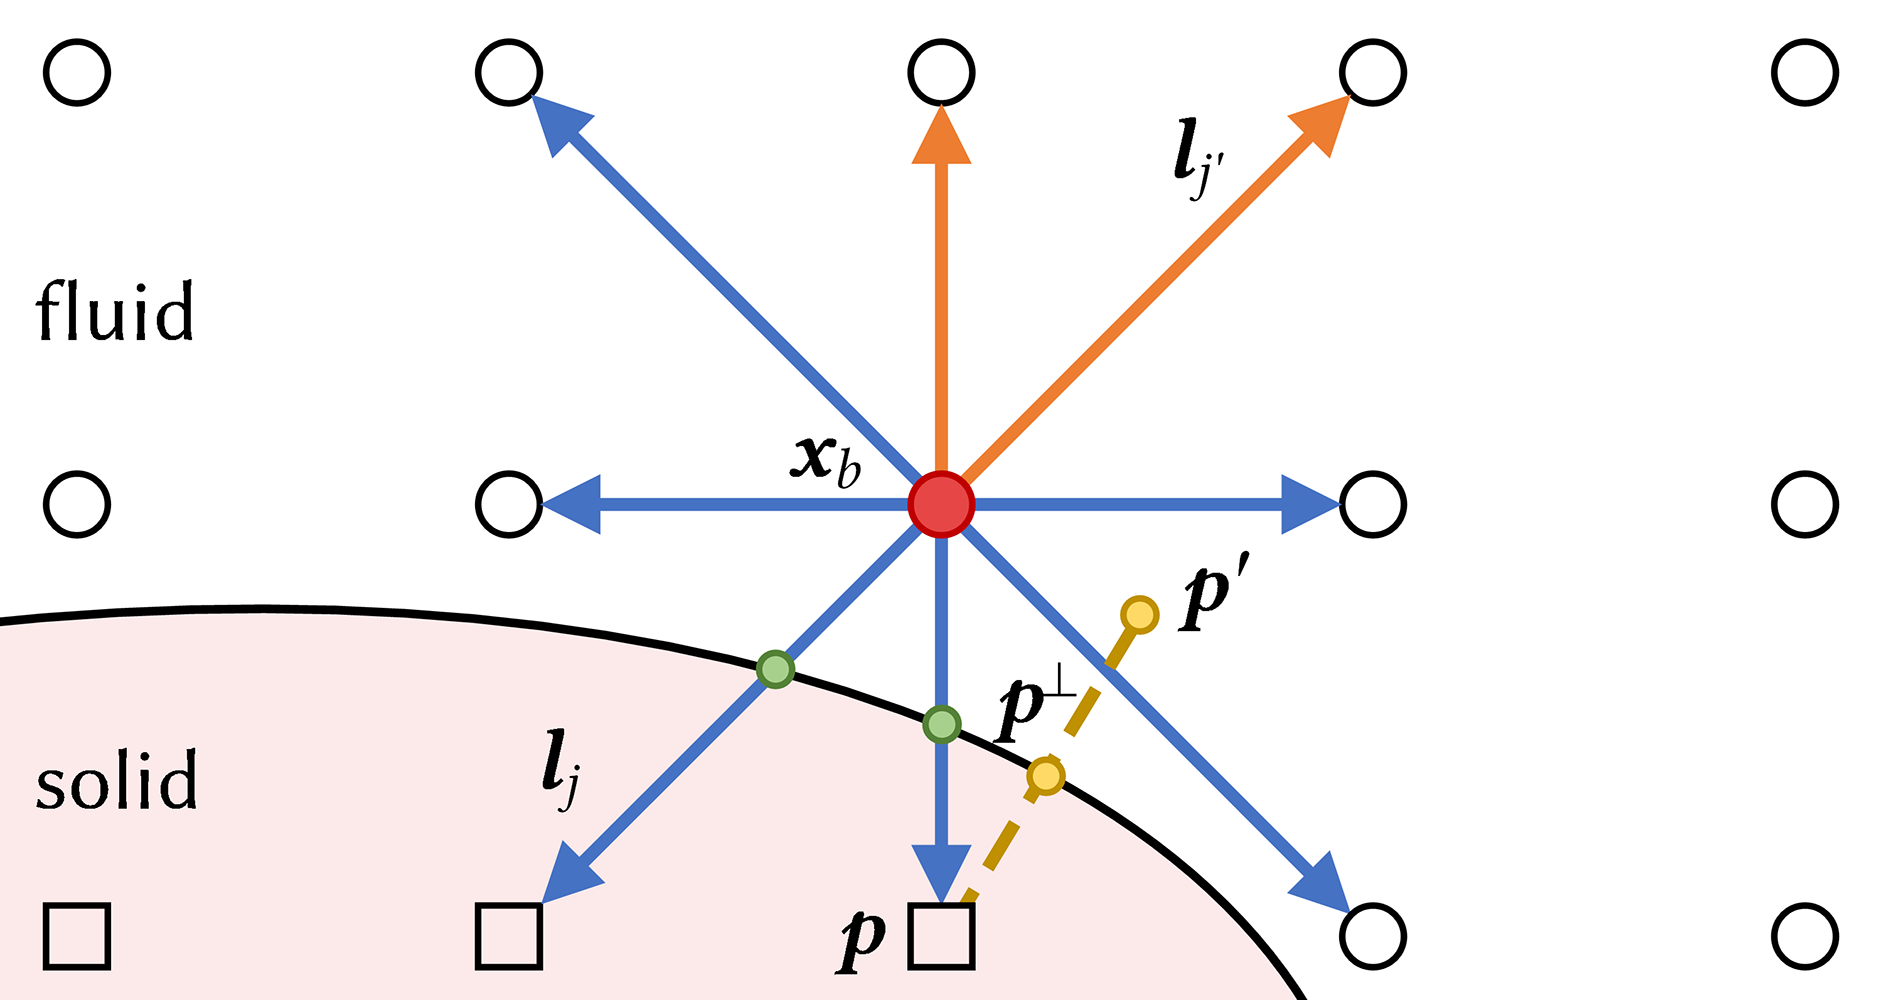
\includegraphics[width=0.75\columnwidth]{figures/bounce_back_scheme.png}
    \bicaption{固体边界的简单反弹方法与锐利界面浸入边界法。在迁移过程中,固体边界附近的流体格点$\bm{x}_b$ (图中标为红色圆圈) 的一部分分布函数$f_{j'}$ (图中标为橘色箭头) 是未知的,因为格点$\bm{x}_b-\bm{l}_{j'}$在固体内部 (图中标为方框),从而需要使用线段$\bm{x}_b$至$\bm{x}_b-\bm{l}_{j'}$与边界的交点 (图中标为绿色圆圈) 的速度$\bm{u}_s$来实现简单反弹边界处理,或$\bm{p}^\perp$与$\bm{p}'$点来实现锐利界面浸入边界处理。}{Simple bounce-back scheme and sharp-interface immersed boundary near fluid-solid boundary. During streaming, some of the distribution functions $f_{j'}$ (corresponding to the orange links) at the fluid node $\bm{x}_b$ (red circle) near a solid boundary are unknown, since the node at $\bm{x}_b-\bm{l}_{j'}$ is located inside the solid region (shown as boxes), requiring a bounce-back scheme using the velocity $\bm{u}_s$ of the boundary velocity at the intersection point (green circles) between the line segment from $\bm{x}_b$ to $\bm{x}_b-\bm{l}_{j'}$ and the solid boundary, or sharp-interface immersed boundary using $\bm{p}^\perp$ and $\bm{p}'$.}
    \label{img:bounce_back_scheme}
\end{figure}

\subsection{插值反弹边界}
简单反弹边界的一个问题是只有边界在速度方向中点时,边界处理的精度才可达到二阶。边界处于其他位置时,边界处理的精度只有一阶。
针对这一问题,插值反弹边界 (Interpolated bounce-back, IBB) 被提出~\cite{Bouzidi-2001},通过考虑边界到格点的距离,进行分布函数的插值:
\begin{equation}\label{eq:ibb_2001}
    f_i(\mathbf{x}_B, t+1) = 
    \begin{cases}
        2 q f^{*}_{\bar{\imath}}(\mathbf{x}_B, t)+(1-2 q) f^{*}_{\bar{\imath}}(\mathbf{x}_{F}, t), & q < 0.5, \\
        \frac{1}{2 q} f^{*}_{\bar{\imath}}(\mathbf{x}_B, t)+\frac{2 q-1}{2 q} f^{*}_i(\mathbf{x}_B, t), & q \geq 0.5,
    \end{cases}
\end{equation}
其中$q=\|\mathbf{x}_B - \mathbf{x}_W\|/\|\bm{c}_i\|$是边界点到边界的正则化距离。

在引入基于距离的插值后,反弹边界可以达到二阶精度,但是依然有一些问题。首先是公式~\ref{eq:ibb_2001} 引入了邻居点参与计算,对于GPU实现会降低数据访问效率。其次,当处理复杂外形的几何时,格点可能处于两个边界之间,导致找不到邻居点从而无法完成边界处理。最后,如第~\ref{sec:1_related_works_LBM} 节所介绍的,IBB在Bouzidi等~(\citeyear{Bouzidi-2001}) 后成为了一类方法,之后的工作提出了诸多不同的构造形式,甚至参数化的构造。这些不同的构造的性能与精度均有所区别。关于这一部分我们将在第\ref{sec:sig23}章中继续讨论。

\makebiblio

\backmatter
\begin{acknowledgement}
    感谢上海科技大学,让我真正感受到了大学的魅力。

    感谢我的导师刘晓培教授,对资质驽钝的我不倦教导,才令我得以小有所成。

    感谢Mathieu Desbrun与郑昌熙教授,能与您二位合作并建立友谊是我莫大的荣幸。

    感谢所有帮助过我、教导过我的老师们。我在上课时总是走神,所以你们的智慧和知识我尚只得其万一,但依然是我这一生宝贵的财富。

    感谢上海科技大学FLARE实验室的全体成员,尤其我的师兄,李伟博士与柏凯博士。每次与你们交流都使我受益匪浅。
\end{acknowledgement}

\ifgraduate
\begin{resume}
  李润东,\shtthesis{} 项目初版作者及维护者,热爱摸鱼。
\end{resume}

\begin{publications}
  论文发表…… (非匿名环境)
\end{publications}

\begin{publications*}
  论文发表…… (匿名环境)
\end{publications*}

\begin{patents}
  专利申请或授权记录…… (非匿名环境)
\end{patents}

\begin{patents*}
  专利申请或授权记录…… (匿名环境)
\end{patents*}

\begin{projects}
  个人参与的科研项目、获奖情况…… (仅非匿名环境显示)
\end{projects}
\fi

\end{document}
